% MASTER'S THESIS — modular LaTeX starter (adapted from shared template)
% Build: latexmk -pdf main.tex
\documentclass[a4paper,12pt,oneside,openany]{book}
% EDIT THIS FILE FIRST. Keep personal data out of AGENTS.md and Git history if desired.
\newcommand{\ThesisUniversity}{Universit\`a degli Studi di Padova}
\newcommand{\ThesisDepartment}{Department of Physics and Astronomy ``Galileo Galilei''}
\newcommand{\ThesisDegree}{Master's Degree in Physics of Data}
\newcommand{\ThesisType}{Master's Thesis}
\newcommand{\ThesisTitle}{Towards lightweight AI Models for Anomaly Detection in Satellite Telemetry Data}
\newcommand{\ThesisCandidate}{Dario Liotta}
\newcommand{\ThesisSupervisor}{Jacopo Pazzini}
\newcommand{\ThesisCoSupervisor}{Tiziano Zingales}
\newcommand{\ThesisAcademicYear}{2025/2026}

% Enable once references.bib has real, cited entries.
\newif\ifthesisbibliography
\thesisbibliographyfalse % switch to \thesisbibliographytrue

\thesisbibliographytrue
% preamble/preamble.tex — packages and global settings

% --- Encoding, fonts, language ---
\usepackage[T1]{fontenc}
\usepackage[utf8]{inputenc}
\usepackage[english]{babel}
\usepackage{lmodern}
\usepackage{microtype}

% --- Page layout ---
% Top and bottom margins generous (2cm left/right keep the 17cm text block
% the TikZ figures are drawn against).
\usepackage[a4paper,top=3cm,bottom=3cm,left=2cm,right=2cm,headheight=15pt,headsep=0.6cm]{geometry}
\usepackage{setspace}

% --- Running header: subsection left, chapter
% right, small italic over a rule; page number bottom centre. Chapter
% openings keep the plain style (no header, number at the bottom).
% Titles are not uppercased, preserving technical capitalization.
\usepackage{fancyhdr}
\pagestyle{fancy}
\fancyhf{}
\fancyhead[L]{\small\itshape\nouppercase{\rightmark}}
\fancyhead[R]{\small\itshape\nouppercase{\leftmark}}
% Page number in footer (oneside layout).
\fancyfoot[R]{\thepage}
\renewcommand{\headrulewidth}{0.4pt}
\fancypagestyle{plain}{%
  \fancyhf{}%
  \fancyfoot[R]{\thepage}%
  \renewcommand{\headrulewidth}{0pt}%
}
% Paragraph separation: keep the first-line indent, add a small vertical skip
% between paragraphs so consecutive paragraphs do not read as a wall of text.
\setlength{\parskip}{0.5em}

% --- Math ---
\usepackage{amsmath,amssymb}
\usepackage{mathtools}
\usepackage{upgreek}

% --- Theorem-like environments (formal definitions) ---
\usepackage{amsthm}
\theoremstyle{definition}
\newtheorem{definition}{Definition}[chapter]
\DeclarePairedDelimiter\abs{\lvert}{\rvert}
\newcommand{\dd}{\,\mathrm{d}}

% --- Units and numbers ---
\usepackage{siunitx}
\sisetup{per-mode=symbol}

% --- Graphics, floats, tables ---
\usepackage{graphicx}
\graphicspath{{figures/}}
\usepackage{float}
\usepackage{placeins}
\usepackage{subfig}
\usepackage{tikz}
\usetikzlibrary{arrows.meta,positioning,calc,fit}
\usepackage{pgfplots}
\pgfplotsset{compat=1.18}
\usepgfplotslibrary{groupplots}
\usepackage[font=small,labelfont=bf]{caption}
\usepackage{booktabs}
\usepackage{multirow}
\usepackage{tabularx}
\usepackage{listings}

% --- Source code listing style ---
\lstdefinestyle{thesiscode}{
  basicstyle=\ttfamily\footnotesize,
  keywordstyle=\bfseries,
  commentstyle=\itshape,
  stringstyle=\ttfamily,
  showstringspaces=false,
  keepspaces=true,
  columns=fullflexible,
  frame=single,
  rulecolor=\color{black!20},
  aboveskip=6pt,
  belowskip=6pt,
  captionpos=b,
  floatplacement=htbp
}

% --- Miscellaneous ---
\usepackage{xcolor}
\usepackage{titlesec}
\usepackage{xspace}
\usepackage{enumitem}
\usepackage{chemformula}
\usepackage{comment}
\usepackage{eso-pic}
\usepackage{transparent}
\usepackage{indentfirst}
\usepackage{setspace}

% --- Chapter heading style ---
\titleformat{\chapter}[display]
  {\normalfont\huge\bfseries}
  {\filleft\huge\chaptertitlename~\thechapter}
  {3ex}
  {\vspace{1.5ex}\filright}
  [\vspace{1ex}\titlerule]

% --- Abbreviations (macros + list of abbreviations) ---
% The list heading is typeset in main.tex (so it lands in the ToC), hence
% heading = none here. Default display = used: only acronyms that appear in
% the text are listed.
\usepackage{acro}[=v3]
\acsetup{list/heading = none}
% Declare only acronyms actually needed by the thesis; expand at first use.
\DeclareAcronym{AD}{short = AD, long = Anomaly Detection}
\DeclareAcronym{GPU}{short = GPU, long = Graphics Processing Unit}
\DeclareAcronym{FPGA}{short = FPGA, long = Field-Programmable Gate Array}
\DeclareAcronym{HLS}{short = HLS, long = High-Level Synthesis}
\DeclareAcronym{MTS}{short = MTS, long = Multivariate Time Series}
\DeclareAcronym{POT}{short = POT, long = Peaks over Threshold}
\DeclareAcronym{PR}{short = PR, long = Precision--Recall}
\DeclareAcronym{ROC}{short = ROC, long = Receiver Operating Characteristic}
\DeclareAcronym{SMD}{short = SMD, long = Server Machine Dataset}
\DeclareAcronym{SMAP}{short = SMAP, long = Soil Moisture Active Passive}
\DeclareAcronym{OPS-SAT}{short = OPS-SAT, long = Operations Satellite}
\DeclareAcronym{ESA}{short = ESA, long = European Space Agency}
\DeclareAcronym{NASA}{short = NASA, long = National Aeronautics and Space Administration}
\DeclareAcronym{MSL}{short = MSL, long = Mars Science Laboratory}
\DeclareAcronym{TOAST}{short = TOAST, long = Transformers On-Board for Anomaly-detection in Satellite Telemetry}


% --- Hyperlinks (keep last) ---
\usepackage[colorlinks,allcolors=blue!50!black]{hyperref}
\hypersetup{linktocpage}

\begin{document}
\hypersetup{pageanchor=false}
\frontmatter

% ==========================================
% TITLE PAGE
% ==========================================

\begin{titlepage}
\thispagestyle{empty}

% ==========================================
% BACKGROUND WATERMARK — VERSION C
% Grande, spostato a sinistra e parziale
% ==========================================
\AddToShipoutPictureBG*{%
  \put(\LenToUnit{0.08\paperwidth},
       \LenToUnit{0.50\paperheight}){%
    \makebox(0,0){%
      \transparent{0.075}%
      
\includegraphics[
        width=1.15\paperwidth,
        keepaspectratio
      ]{figures/logounipdgrigio.png}%
    }%
  }%
}

% ==========================================
% HEADER
% ==========================================
\begin{center}

\vspace*{2mm}


\includegraphics[
  height=25mm,
  keepaspectratio
]{figures/Logo_Universita_Padova.png}

\vspace{7mm}

{\LARGE\scshape
 \ThesisUniversity\par}

\vspace{4mm}

{\large\bfseries
 \ThesisDepartment\par}

\vspace{3mm}

{\large
 \ThesisDegree\par}

% ==========================================
% THESIS TYPE
% ==========================================
\vspace{12mm}

{\Large\scshape
 \ThesisType\par}

% ==========================================
% THESIS TITLE
% ==========================================
\vspace{18mm}

\makebox[\textwidth][c]{%
  \begin{minipage}{1.10\textwidth}
    \centering
    {\fontsize{21}{26}\selectfont
     \bfseries
     \ThesisTitle\par}
  \end{minipage}%
}

\end{center}

% ==========================================
% FLEXIBLE VERTICAL SPACE
% ==========================================
\vfill

% ==========================================
% SUPERVISOR AND CANDIDATE
% ==========================================
\noindent
\begin{minipage}[t]{0.46\textwidth}
  \raggedright

  {\large\bfseries Supervisor\par}

  \vspace{3mm}

  {\Large \ThesisSupervisor\par}

\end{minipage}%
\hfill
\begin{minipage}[t]{0.46\textwidth}
  \raggedleft

  {\large\bfseries Candidate\par}

  \vspace{3mm}

  {\Large \ThesisCandidate\par}

\end{minipage}

% ==========================================
% ACADEMIC YEAR
% ==========================================
\vspace{17mm}

\begin{center}
  {\large\bfseries
   Academic Year \ThesisAcademicYear\par}
\end{center}

\vspace*{1mm}

\end{titlepage}

\clearpage{\pagestyle{empty}\cleardoublepage}

\hypersetup{pageanchor=true}
\chapter*{Abstract}
\phantomsection
\addcontentsline{toc}{chapter}{Abstract}
% Abstract to be written after the experimental results are finalized.

\tableofcontents
\chapter*{List of Abbreviations}
\phantomsection
\addcontentsline{toc}{chapter}{List of Abbreviations}
\printacronyms
\chapter*{Acknowledgements}
\phantomsection
\addcontentsline{toc}{chapter}{Acknowledgements}
% Acknowledgements to be added by the author.

\mainmatter
% To compile only selected chapters, uncomment one line before the includes:
% \includeonly{chapters/chapter-introduction}
\chapter{Introduction}
\label{chap:introduction}

% Draft requested by the author on 2026-11-05. Scope follows outline.md.
% Literature claims are cited below; no experimental performance numbers are
% introduced in this chapter. Experimental provenance is recorded in the journal.

\section{Satellite telemetry and anomaly detection}
\label{sec:introduction-telemetry}

Satellite telemetry consists of measurements collected from spacecraft sensors
and subsystems. These data, among other things, help operators monitor the spacecraft and identify
unexpected behavior~\cite{Hundman2018Spacecraft}. This thesis studies lightweight
models for anomaly detection, with future onboard use as the target application.
The aim is to support the analysis of telemetry directly on the satellite,
where memory and computing resources are limited~\cite{TOASTExecutiveSummary}.

Traditional monitoring relies on limits assigned to individual telemetry
parameters, and an alert is generated when a measurement exceeds these limits.
However, some anomalies occur within the allowed ranges and can only be
identified by considering how the signal changes over time. The expected behavior
also depends on some operating conditions and spacecraft
commands~\cite{Hundman2018Spacecraft}. Models that learn from past telemetry
provide another way to detect these changes: they produce an anomaly score
for each observation, and a threshold determines whether an observation is
classified as anomalous~\cite{Yermakov2025TranADPlus}.

An anomaly is a signal that requires attention, but it does not necessarily
identify a fault or explain its cause. In the \ac{OPS-SAT} benchmark,
telemetry segments were selected and labeled by spacecraft operations
engineers and machine learning experts. Segments were considered anomalous
when their behavior required operators to be notified. Examples include
unexpected peaks, unusual signal shapes, zero values and gaps in the
measurements~\cite{Ruszczak2025OPSSAT}.

Onboard anomaly detection is particularly relevant when communication with
the ground is limited. Downlink capacity restricts the amount of telemetry
that can be transmitted, while gaps in ground contact can delay its analysis.
Processing data onboard could help identify relevant events and select the
information to transmit. This is a motivation of the \ac{TOAST} project,
within which this thesis is developed~\cite{TOASTExecutiveSummary}.
The models considered here must therefore be assessed both for their detection
performance and for the resources required to run them.

\section{Towards lightweight models for onboard inference}
\label{sec:introduction-lightweight}

Running a neural network onboard requires memory to store its weights
and intermediate results, as well as computing resources to process each
input. Moving data between memory and the processor also contributes to
execution time and energy consumption. A reduction in the number of
operations does not therefore guarantee a proportional reduction in
execution time: the result also depends on the hardware and its
implementation~\cite{Sze2017EfficientDNN}.

In this thesis, the term \emph{lightweight} refers to models with lower
storage or computational requirements than a reference model. We will compare
the number of trainable parameters, the memory needed to store the model and
the estimated number of operations.
These quantities are considered together with detection performance
to assess which changes provide a useful reduction in resource requirements.

The reference model considered here is based on transformers. Their attention
mechanism combines information from different positions in an input
sequence~\cite{Vaswani2017Attention}, and this allows a model to use relationships
between observations at different times. TranAD applies this architecture
to anomaly detection in multivariate time series~\cite{Tuli2022TranAD}, while
TranAD+ builds on top of TranAD and evaluates a modified implementation on
several anomaly-detection benchmarks~\cite{Yermakov2025TranADPlus}.

We use TranAD+ as the reference model for our experiments. In the
implementation used here, the model receives a window of observations
and reconstructs its last sample, so that the reconstruction error is then used
to calculate an anomaly score. Effective detection requires this score
to distinguish nominal from anomalous observations. A lower reconstruction
error alone does not guarantee better anomaly detection, because errors
can decrease for both types of observation.

We study several ways to simplify the model: reducing the window size
limits the amount of past data processed for each observation; reducing
the feed-forward dimension makes the internal layers smaller;
architectural changes remove or reuse parts of the reference model;
quantization reduces the numerical precision
used to represent weights and to perform
calculations~\cite{Sze2017EfficientDNN}. For each change, we evaluate
both the reduction in resource requirements and its effect on
anomaly detection. We also compare TranAD+ with lightweight detectors
that do not use transformers and operate on simple statistics of the
signal.

\section{The TOAST project and thesis scope}
\label{sec:introduction-toast}

\ac{TOAST} is a research proposal at the University of Padua, involving
the Department of Physics and Astronomy and the Department of Information
Engineering. It aims to develop compact transformer models for onboard
anomaly detection in satellite telemetry. The project also plans their
implementation on embedded devices and the assessment of their robustness
against faults caused by radiation~\cite{TOASTExecutiveSummary}.

This thesis contributes to the model-development part of the proposal.
We first assess the reproducibility of TranAD+ on the benchmarks
considered in its original study~\cite{Yermakov2025TranADPlus},
and then investigate changes to the model and evaluate their effects
on detection performance and resource requirements. Finally, we consider
whether a detector without transformers can meet the same requirements,
since the choice of model for onboard use should follow from the evidence.

The main dataset is \ac{OPS-SAT}, which contains telemetry from an
experimental CubeSat operated by the \ac{ESA}. The data are organized
into single-channel signal fragments, each labeled as nominal or
anomalous~\cite{Ruszczak2025OPSSAT}. We use the measurements
within each fragment as a sequence of inputs with one feature.

The experiments in this thesis assess trained models through software
execution on the available computing platform. They provide information
about detection performance and computational requirements that can
support future onboard deployment. Implementation on embedded hardware
and radiation testing belong to later stages of the broader
\ac{TOAST} proposal~\cite{TOASTExecutiveSummary}.

\section{Objectives and research questions}
\label{sec:introduction-questions}

The objective of this thesis is to investigate how a transformer-based
anomaly detector can be simplified, and how these changes affect detection
performance and resource requirements. We start from TranAD+ as a reference
and study changes to its input window, internal dimensions, architecture
and numerical precision. The work addresses the following research questions:

\begin{enumerate}[label=\arabic*.]
  \item \textbf{Reference reproducibility.}
  How closely can we reproduce the published TranAD+ results using
  the available code, the same configurations and evaluation procedures?

  \item \textbf{Window size and feed-forward dimension.}
  How do changes to the input window and feed-forward dimension inside the transformer affect
  model performance?

  \item \textbf{Architectural simplification.}
  Can parts of the reference model be removed or shared while retaining
  detection performance?

  \item \textbf{Quantization.}
  How much can quantization reduce model storage, and how does it affect
  detection performance? What results are obtained with quantized weights
  and with integer matrix operations?

  \item \textbf{Evaluation protocol.}
  Do the metrics of the reference evaluation procedure distinguish
  models that separate anomalous from nominal observations from models
  that do not?

  \item \textbf{Lightweight alternatives.}
  Can a detector without transformers, based on simple statistics
  of the signal, provide better anomaly detection with lower resource
  requirements?
\end{enumerate}

The benchmark reproduction establishes a reference for the subsequent
comparisons. The evaluation procedure must also be considered, since
detection scores depend, for example, on how thresholds are selected.

These experiments test which resource reductions can be achieved
without losing detection capability, and whether they can also improve
detection performance. The direction and
size of each effect must therefore be established from the results.

For the model-comparison studies, repeated training runs are used
to assess sensitivity to random initialization and other random
operations during training. Comparisons use corresponding seeds,
and average performance is reported together with its variability:
this helps distinguish consistent effects from differences that
depend on an individual run.

\section{Contributions and organization of the thesis}
\label{sec:introduction-contributions}

As already stated, this thesis provides an experimental study of model simplification
for anomaly detection in satellite telemetry. We start from
the reproduction of TranAD+ benchmarks and its adaptation to
\ac{OPS-SAT}.

The subsequent experiments examine changes to window size,
feed-forward dimension, model architecture and numerical precision.
The architectural variants include a shared decoder, a single
encoder--decoder pass and an encoder followed by a reconstruction head.
Quantization is then evaluated using
the corresponding trained models as references. We also examine the
evaluation procedure itself and compare TranAD+ with lightweight
detectors without transformers.

The remaining chapters are organized as follows.
Chapter~\ref{chap:background} introduces time-series anomaly detection,
transformers, TranAD and TranAD+: it explains the model components
considered in the experiments and introduces lightweight detectors
without transformers.

Chapter~\ref{chap:datasets} presents the datasets, preprocessing,
training and evaluation procedures. It also describes anomaly scores,
threshold selection, point adjustment and the quantities used to assess
resource requirements.

Chapter~\ref{chap:replication} examines the reproduction of the
TranAD+ benchmarks and the adaptation to \ac{OPS-SAT}:
it discusses the differences between the reproduced and published
results and the checks performed to investigate them.

Chapter~\ref{chap:ablation} studies the effects of changing window size
and feed-forward dimension, both separately and together, while Chapter~\ref{chap:architecture}
presents the architectural variants
and Chapter~\ref{chap:quantization} shows quantization experiments, comparing detection performance
with resource requirements.

Chapter~\ref{chap:conclusions} discusses the main findings,
their limitations and possible developments within \ac{TOAST}.

\chapter{Reference Models}
\label{chap:background}
\chaptermark{Reference Models}

% First draft requested by the author on 2026-11-05.
% Mathematical definitions are literature-backed or explicit descriptions of
% the pinned reference implementation. No experimental results are introduced.

\section{Anomaly detection in time series}
\label{sec:background-anomalies}
An anomaly is an observation, or a group of observations, that departs from
the behavior considered normal for the system under study. This definition
depends on the application: a statistical deviation becomes relevant when it
conflicts with the expected operation of the system. For telemetry, the
reference behavior can depend on operating modes, commands and temporal
relationships among measurements~\cite{Chandola2009AnomalySurvey,Hundman2018Spacecraft}.

We represent an observation at time index \(t\) by a row vector
\(\mathbf{x}_t\in\mathbb{R}^{F}\), where \(F\) is the number of numerical input
features. A univariate series has \(F=1\); a multivariate series has \(F>1\).
Features can include measured quantities and numerical encodings of additional
information. Their units and scales must be considered before combining them
in a reconstruction error. In the following model equations, inputs are
normalized and the corresponding errors are dimensionless.

A finite temporal context is supplied through the sliding window defined in
Equation~\eqref{eq:background-window}:
\begin{equation}
  \mathbf{W}_t =
  \begin{bmatrix}
    \mathbf{x}_{t-w+1}\\
    \vdots\\
    \mathbf{x}_{t}
  \end{bmatrix}
  \in \mathbb{R}^{w\times F}.
  \label{eq:background-window}
\end{equation}
Here, \(w\) is the window length in samples and \(\mathbf{W}_t\) contains the
observations ending at index \(t\). Its rows are samples and its columns are
features. Padding conventions for the beginning of a series, and the treatment
of separate telemetry fragments, are specified in Chapter~\ref{chap:datasets}.
No observation later than \(t\) appears in this window.

Anomalies are commonly classified as point, contextual or
collective~\cite{Chandola2009AnomalySurvey}. A point anomaly is an individual
observation that is unusual relative to the reference distribution. A
contextual anomaly is unusual only within a specified context; for example, a
sensor value can be plausible during a maneuver but unexpected during a stable
operating period. A collective anomaly is a sequence whose joint behavior is
unusual, even if its individual values are not. A persistent constant reading
can belong to this category when normal behavior requires variation. These
categories describe different aspects of an event and need not be exclusive.

Models can learn the expected behavior of a system from nominal
observations and identify anomalies by comparing their outputs
with the observed measurements~\cite{Hundman2018Spacecraft}.
A reconstruction loss does not require anomaly labels, but the
training data can still be selected as nominal.

The annotation granularity is a separate issue. A point label identifies the
status assigned to a sample, whereas a fragment label describes an interval as
a whole. The \ac{OPS-SAT} data discussed in Chapter~\ref{chap:introduction}
provide fragment annotations~\cite{Ruszczak2025OPSSAT}. Repeating such a label
on every sample makes pointwise calculations possible, but does not supply a
measured anomaly onset within that fragment.

\section{Reconstruction-based detection and anomaly scores}
\label{sec:background-reconstruction}

A reconstruction model learns to reproduce observed data.
In an autoencoder, an encoder maps the input to an internal
representation, and a decoder uses this representation to
reconstruct the input~\cite{Goodfellow2016DeepLearning}.
The reconstruction error can then be used as an anomaly
score~\cite{Tuli2022TranAD}.
It is important to state the underlying assumption: a model trained on nominal data
will reconstruct nominal observations more accurately than
anomalous ones.

In the implementation used here, the model receives the window
$\mathbf{W}_t$ and reconstructs its last sample
$\mathbf{x}_t$~\cite{TranADPlusReferenceCode}.
We describe this mapping as

\begin{equation}
  \widehat{\mathbf{x}}_t = f_{\theta}(\mathbf{W}_t).
  \label{eq:background-reconstruction}
\end{equation}

Here, $f_{\theta}$ represents the model with trainable parameters
$\theta$, while $\widehat{\mathbf{x}}_t$ is the reconstructed sample.
The target $\mathbf{x}_t$ is already included in the input window.
This means that the task is therefore to reconstruct an observed value, rather than
predict a future one.

We calculate the anomaly score as the mean squared reconstruction
error across the input features:

\begin{equation}
  s_t = \frac{1}{F}\sum_{j=1}^{F}
  \left(\widehat{x}_{t,j}-x_{t,j}\right)^2.
  \label{eq:background-mse-score}
\end{equation}

Here, $F$ is the number of features, while $x_{t,j}$ and
$\widehat{x}_{t,j}$ are the observed and reconstructed values
of feature $j$. The inputs are normalized before processing:
the reference implementation rescales each feature with the minimum
and maximum of the training data, without clipping~\cite{TranADPlusReferenceCode}.
Test observations can therefore fall outside the interval $[0,1]$,
whereas the output layer of TranAD+ (Section~\ref{sec:background-tranadplus})
is restricted to this interval.
Averaging the errors produces a single score for each sample,
following the approach described in
TranAD+~\cite{Yermakov2025TranADPlus}.

It is important to keep in mind that an
autoencoder with sufficient capacity can learn to copy its
inputs without learning useful properties of the
data~\cite{Goodfellow2016DeepLearning}.
For anomaly detection, accurate reconstruction is useful only
if the resulting scores distinguish nominal from anomalous
observations. Small reconstruction errors alone do not guarantee
this distinction.

A threshold converts the score into a binary prediction:

\begin{equation}
  \widehat{y}_t = \mathbb{1}\!\left[s_t>\tau\right].
  \label{eq:background-threshold}
\end{equation}

Here, $\tau$ is the threshold and $\mathbb{1}$ is the indicator
function. The predicted label $\widehat{y}_t$ is $1$ when the score
exceeds the threshold and $0$ otherwise.

Changing the threshold changes the predictions without changing
the trained model. Post-processing can also change the reported
metrics without changing the reconstruction errors.

\section{TranAD}
\label{sec:background-tranad}

TranAD is a transformer-based model developed for anomaly detection
in multivariate time series~\cite{Tuli2022TranAD}.
Its reconstruction process uses attention to combine information
from different positions in a sequence, with weights calculated
from the input representations~\cite{Vaswani2017Attention}.
Self-attention relates positions within the same sequence, while
cross-attention uses information from another sequence.

In an encoder--decoder architecture, the encoder builds internal
representations of the input, which the decoder uses to produce
an output. Attention is combined with feed-forward layers that
apply the same transformation separately at each sequence position;
their intermediate width is called the feed-forward dimension.
Positional information is also supplied so that the model can
account for the order of the samples~\cite{Vaswani2017Attention}.

The published TranAD architecture combines a representation of
the history up to the current time with a local input window.
A complete-sequence encoder processes the history, while a window
encoder combines local information with this broader context.
Two decoders produce reconstructions, as shown in
Figure~\ref{fig:background-tranad}~\cite{Tuli2022TranAD}.

\begin{figure}[htbp]
  \centering
  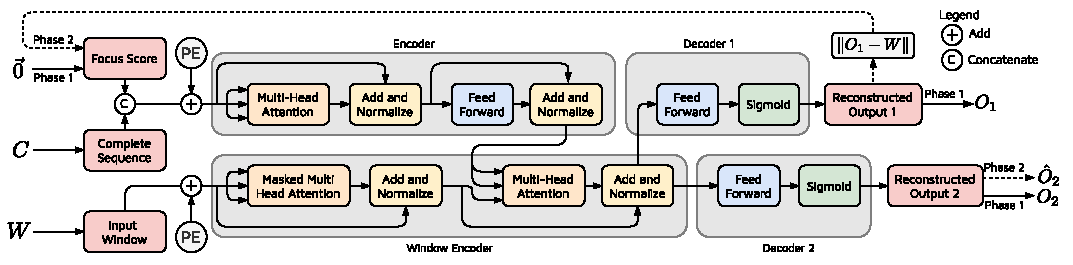
\includegraphics[width=\linewidth]{chapter2/tranad-original.pdf}
  \caption{TranAD architecture, reproduced from Figure 1
  of Tuli et al.~\cite{Tuli2022TranAD}.
  \(C\) denotes the available history, \(W\) the input window,
  and PE the positional encoding.}
  \label{fig:background-tranad}
\end{figure}
% Source: docs/papers/TranAD.pdf, Fig. 1, printed p. 1204 / PDF p. 4.

Reconstruction takes place in two phases: the first produces
an initial reconstruction, whose error becomes a focus signal
for the second. This process, called \textit{self-conditioning}, allows
the second reconstruction to depend on the errors found
in the first, without requiring anomaly labels.

The published training procedure combines reconstruction losses
with an adversarial objective, in which the two decoders have
opposing objectives for the second-phase reconstruction
error~\cite{Tuli2022TranAD}.

\section{TranAD+}
\label{sec:background-tranadplus}

\subsection{Reference architecture and training objective}
\label{sec:background-tranadplus-training}

The reference model used in this thesis is TranAD+, introduced
by Yermakov et al. and built on TranAD for anomaly detection
in high-bandwidth satellite communications~\cite{Yermakov2025TranADPlus}.
The work is motivated by DSN monitoring data, which contain
numerical and categorical variables as well as missing values.
The aim is to support operations engineers in monitoring increasing
amounts of incoming data by adapting the preprocessing and the
model to these inputs~\cite{Yermakov2025TranADPlus}.
Among other things, the original training pipeline selected only
one track for each of the SMAP, MSL and SMD datasets, while TranAD+
uses all tracks in the training
split~\cite{TranADReferenceCode,TranADPlusReferenceCode}.

The model contains a transformer encoder, two transformer decoders
and an output layer consisting of a linear transformation followed
by a sigmoid. The same encoder and output layer are used in both
processing passes, while the two decoders have separate parameters.
Figure~\ref{fig:background-tranadplus-flow} shows these components
and their connections.

\begin{figure}[htbp]
  \centering
  % Source: original TranAD+ Fig. 1 for topology; models.py:34--60 and
  % helpers.py:667--670 for exact sharing, focus and current-point query.
  \begin{tikzpicture}[
    x=1cm,y=1cm,>=Stealth,font=\small,
    block/.style={draw,rounded corners=2pt,align=center,
      minimum height=1.05cm,inner sep=5pt},
    input/.style={block,fill=black!8,minimum width=2.6cm},
    encoder/.style={block,fill=blue!10,minimum width=2.2cm},
    decoder/.style={block,fill=black!12,minimum width=2.5cm},
    head/.style={block,fill=blue!10,minimum width=2.4cm},
    output/.style={block,fill=black!8,minimum width=2.6cm},
    data/.style={->,semithick},
    sharing/.style={dashed,black!65},
    feedback/.style={->,dashed,semithick},
    note/.style={font=\footnotesize,fill=white,inner sep=2pt}
  ]
    \node[input] (in1) at (1.30,0)
      {Window $\mathbf{W}_t$\\Zero focus $\mathbf{0}$};
    \node[encoder] (en1) at (4.55,0) {Encoder\\$E$};
    \node[decoder] (de1) at (7.60,0)
      {Decoder $D_1$\\query $\mathbf{q}_t$};
    \node[head] (hd1) at (10.70,0) {Output head\\$P$};
    \node[output] (ou1) at (14.00,0)
      {Reconstruction\\$\widehat{\mathbf{x}}_t^{(1)}$};

    \node[input] (in2) at (1.30,-2.70)
      {Window $\mathbf{W}_t$\\Focus $\mathbf{C}^{(1)}_t$};
    \node[encoder] (en2) at (4.55,-2.70) {Encoder\\$E$};
    \node[decoder] (de2) at (7.60,-2.70)
      {Decoder $D_2$\\query $\mathbf{q}_t$};
    \node[head] (hd2) at (10.70,-2.70) {Output head\\$P$};
    \node[output] (ou2) at (14.00,-2.70)
      {Reconstruction\\$\widehat{\mathbf{x}}_t^{(2)}$};

    \node[anchor=west,font=\small\bfseries] at (0,0.91) {Pass 1};
    \node[anchor=west,font=\small\bfseries] at (0,-1.79) {Pass 2};
    \foreach \a/\b in {in1/en1,en1/de1,de1/hd1,hd1/ou1,
                       in2/en2,en2/de2,de2/hd2,hd2/ou2}
      \draw[data] (\a) -- (\b);
    \draw[sharing] (en1.south) --
      node[note,midway] {shared weights} (en2.north);
    \draw[sharing] (hd1.south) --
      node[note,midway] {shared weights} (hd2.north);
    \draw[feedback] (ou1.east) -- (15.90,0) -- (15.90,-4.12)
      -- node[note,midway]
      {$C^{(1)}_{t,k,j}=(\widehat{x}_{t,j}^{(1)}-W_{t,k,j})^2$}
      (1.30,-4.12) -- (in2.south);
  \end{tikzpicture}
  \caption{Computation in the TranAD+ reference implementation.
  The repeated \(E\) and \(P\) blocks are calls to the same encoder and
  output head; \(D_1\) and \(D_2\) have separate parameters. The return
  path constructs the focus for the second pass. Each decoder also
  receives the duplicated current sample \(\mathbf{q}_t\). Schematic
  derived from Figure 1 of Yermakov et al.~\cite{Yermakov2025TranADPlus}
  and the inspected implementation~\cite{TranADPlusReferenceCode}.}
  \label{fig:background-tranadplus-flow}
\end{figure}

In the first pass, the encoder receives the input window together
with a matrix of zeros, and the first decoder produces a
reconstruction of the last sample: this reconstruction is then
compared with every sample in the window, using squared differences
to construct the focus matrix. The same encoder processes the
window again with this focus, and the second decoder produces
another reconstruction. Both decoders also receive the current
sample as an input~\cite{TranADPlusReferenceCode}.

During training, the model minimizes a weighted sum of the two
reconstruction errors:

\begin{equation}
  \mathcal{L}_{n} =
  \frac{1}{n}\operatorname{MSE}
  \left(\widehat{\mathbf{x}}^{(1)}_t,\mathbf{x}_t\right)
  +
  \left(1-\frac{1}{n}\right)\operatorname{MSE}
  \left(\widehat{\mathbf{x}}^{(2)}_t,\mathbf{x}_t\right),
  \label{eq:background-tranadplus-loss}
\end{equation}

where $n\geq1$ is the training epoch, while
$\widehat{\mathbf{x}}^{(1)}_t$ and
$\widehat{\mathbf{x}}^{(2)}_t$ are the two reconstructions.
The mean squared error is averaged over features and batch
elements. Only the first reconstruction contributes directly
to the loss in the first epoch; the weight of the second
increases in subsequent epochs~\cite{TranADPlusReferenceCode}.
% Source: TranADPlus/src/helpers.py:831--849; one-based epoch n.

During evaluation, the two reconstructions are combined as

\begin{equation}
  \widehat{\mathbf{x}}_t(\alpha) =
  \alpha\widehat{\mathbf{x}}^{(1)}_t
  +(1-\alpha)\widehat{\mathbf{x}}^{(2)}_t.
  \label{eq:background-tranadplus-combination}
\end{equation}

Here, $\alpha\in[0,1]$ controls the contribution of each
reconstruction. With $\alpha=1$, only the first is used,
while $\alpha=0$ selects the second.
This evaluation parameter is separate from the epoch-dependent
weights used during training~\cite{TranADPlusReferenceCode}.

The combined reconstruction is then compared with the observed
sample to calculate the anomaly score:

\begin{equation}
  s_t(\alpha)=\frac{1}{F}\sum_{j=1}^{F}
  \left[\widehat{x}_{t,j}(\alpha)-x_{t,j}\right]^2.
  \label{eq:background-tranadplus-score}
\end{equation}

The combination therefore takes place before calculating
the squared errors, rather than averaging the errors
of the two reconstructions.
% Source: TranADPlus/src/helpers.py:665--673,726 and scripts/evaluation.py.

\subsection{Changes relative to TranAD}
\label{sec:background-tranadplus-changes}

The main changes concern the feed-forward layers, the combination
of decoder outputs and the training procedure.

\begin{itemize}

  \item TranAD+ introduces an inverse bottleneck in the feed-forward
  layers to limit information loss, particularly with inputs expanded
  by categorical encoding~\cite{Yermakov2025TranADPlus}.
  The transformation first changes the width of the representation
  and then returns it to its initial value:

  \begin{equation}
    d \longrightarrow d_{\mathrm{ff}} \longrightarrow d.
    \label{eq:background-bottleneck}
  \end{equation}

  Here, $d$ is the input and output width, while $d_{\mathrm{ff}}$
  is the intermediate width. A bottleneck makes the intermediate
  representation smaller, whereas an inverse bottleneck makes it
  larger. In the implementation used here, $d=2F$ because the window
  and focus are concatenated, so an expansion occurs when
  $d_{\mathrm{ff}}>2F$~\cite{TranADPlusReferenceCode}.

  \item TranAD+ combines the two reconstructed outputs using
  adjustable weights before calculating the anomaly score.
  The coefficient $\alpha$ controls their contributions, as described
  in Equation~\eqref{eq:background-tranadplus-combination}, allowing
  the score to use either reconstruction or a combination of
  both~\cite{Yermakov2025TranADPlus,TranADPlusReferenceCode}.

  \item Unlike the adversarial training described in the TranAD
  paper, the TranAD+ implementation minimizes a weighted sum
  of reconstruction errors with non-negative weights, as given
  in Equation~\eqref{eq:background-tranadplus-loss}.
  The second reconstruction is therefore trained to reduce its
  error, rather than to increase it through an adversarial
  objective~\cite{Tuli2022TranAD,TranADPlusReferenceCode}.

  \item The original TranAD window-conversion routine produces
  two identical initial windows because of its indexing and
  replication padding. TranAD+ corrects this duplication by
  advancing the window through the
  data~\cite{TranADReferenceCode,TranADPlusReferenceCode}.

  \item The window size, feed-forward dimension, number of layers
  and training settings can be configured in the TranAD+ pipeline.
  The documentation of the reference code also states that the training
  hyperparameters were optimized~\cite{TranADPlusReferenceCode}.
  % Source: TranADPlus/README_original.md:130.

\end{itemize}

\section{Model simplification and resource-aware inference}
\label{sec:background-efficiency}

The attention and reconstruction stages described for TranAD and
TranAD+ require memory to store the model and its intermediate
representations, as well as computation to process each telemetry
window. Starting from TranAD+ as the reference, this thesis therefore
considers detection performance together with these requirements,
since future onboard use depends on the resources available
on the spacecraft.

The number of parameters provides an initial measure of model size,
but the memory needed to store them also depends on their numerical
precision, while inference requires additional space for inputs and
intermediate results~\cite{Sze2017EfficientDNN}.
The distinction between model size and computation is visible in
TranAD+ itself: its two encoder passes use the same learned weights,
but both require operations to be performed, so sharing parameters
does not remove the cost of executing them~\cite{TranADPlusReferenceCode}.

Execution time also depends on the hardware and software used,
so measurements on the available platform do not directly establish
performance on an onboard device~\cite{Sze2017EfficientDNN}.

\section{Lightweight detectors without transformers}
\label{sec:background-lightweight}

Anomaly detection does not require a sequence model. A simpler approach
describes a piece of signal, such as a fragment or a window, with a few
statistics, for example its standard deviation, range or the size of its
changes between consecutive samples. These statistics are then compared
with those of nominal data. The \ac{OPS-SAT} benchmark follows this approach:
it provides statistical features computed for each fragment and
evaluates several detectors on them, including a nearest-neighbour
detector~\cite{Ruszczak2025OPSSAT}.

A nearest-neighbour detector stores the descriptions of nominal training
pieces and assigns each new piece a score equal to its distance from the
closest stored ones: a piece unlike any nominal example receives a high
score~\cite{Chandola2009AnomalySurvey}. Linear methods instead learn a
low-dimensional subspace that contains most of the variation of nominal
data, and use the distance from this subspace as the
score~\cite{Chandola2009AnomalySurvey}. An autoencoder built from fully
connected layers is a non-linear counterpart of this idea: it compresses
the description and reconstructs it, and the reconstruction error is the
score~\cite{Goodfellow2016DeepLearning}.

These detectors contain no attention mechanism. A fully connected network
uses only matrix products and simple element-wise functions, so its
memory and computation per decision are small and fixed. We use them as
lightweight alternatives to TranAD+ and as controls for its evaluation.

\chapter{Datasets and Experimental Protocol}
\label{chap:datasets}
\chaptermark{Datasets and protocol}

% Draft requested by the author on 2026-11-06. Dataset counts are computed
% from the released files, not inferred from benchmark tables. See journal.
This chapter defines the data and experimental procedures used to reproduce
TranAD+ and study its simplification. Dataset properties are separated from
choices made in the implementation. This distinction is necessary because a
change in preprocessing, score construction or evaluation can change a metric
without changing the trained network.

The same reconstruction principle is applied to the three main datasets, but
the available annotations differ. We therefore distinguish the model output,
which is an error for each evaluated sample, from the unit on which detection
is assessed. We also separate evaluations that use test labels to optimize a
score from scoring settings selected on validation data and subsequently
applied to test fragments.

\section{Dataset selection and roles in the study}
\label{sec:datasets-roles}
The experimental work has two related purposes. The first is to reconstruct
the reference results on the six datasets considered in the TranAD+
paper~\cite{Yermakov2025TranADPlus}. The second is to investigate model cost
and detection performance on a smaller set relevant to spacecraft telemetry.
The datasets and their roles are listed in Table~\ref{tab:datasets-roles}.

\begin{table}[htbp]
  \centering
  \small
  \begin{tabularx}{\textwidth}{@{}lXX@{}}
    \toprule
    Dataset & Data source & Role in this thesis \\
    \midrule
    \acs{OPS-SAT} & Satellite telemetry fragments & Reference application and main simplification study \\
    \acs{SMAP} & Earth-observation satellite telemetry and command inputs & Benchmark reproduction and main simplification study \\
    \acs{MSL} & Mars rover telemetry and command inputs & Benchmark reproduction and main simplification study \\
    \acs{SMD} & Server operating measurements & Benchmark reproduction \\
    SWaT & Water-treatment testbed & Benchmark reproduction \\
    WADI & Water-distribution testbed & Benchmark reproduction \\
    DSN\_1k & Deep Space Network communications monitoring & Benchmark reproduction \\
    \bottomrule
  \end{tabularx}
  \caption{Dataset roles. The six reproduction datasets follow the scope of
  the TranAD+ paper. The main model study uses \acs{OPS-SAT}, \acs{SMAP} and
  \acs{MSL}; their descriptions follow the respective dataset sources.}
  \label{tab:datasets-roles}
\end{table}

\ac{OPS-SAT} is the reference application because its data were collected
on an operational experimental satellite and annotated by spacecraft
operations engineers~\cite{Ruszczak2025OPSSAT}. \ac{SMAP} and \ac{MSL}
provide additional spacecraft telemetry benchmarks already used by
TranAD+~\cite{Hundman2018Spacecraft,Yermakov2025TranADPlus}. \ac{SMAP} is an
Earth-orbiting satellite; \ac{MSL} is the Curiosity rover on Mars. Their common
relevance is spacecraft monitoring, rather than identical platforms,
sensors or operating conditions.

The additional reproduction datasets help assess the reference implementation
across the domains used in the published comparison. They are not included
in the main architecture grid. Their benchmark-specific configurations and
preprocessing decisions are documented in Chapter~\ref{chap:replication} and
Appendix~\ref{app:reproducibility}. Agreement on those datasets does not by
itself establish performance on the \ac{OPS-SAT} application.

\section{OPS-SAT telemetry}
\label{sec:datasets-opssat}
\subsection{Telemetry fragments and annotation granularity}
\label{sec:datasets-opssat-labels}
The \ac{OPS-SAT} benchmark contains \num{2123} telemetry fragments from
\num{9} channels. These comprise \num{3} magnetometer channels and \num{6}
photodiode channels. The fragments were selected and annotated through a
process involving spacecraft operations engineers and machine learning
researchers~\cite{Ruszczak2025OPSSAT}. They have varying lengths and sampling
frequencies. The released benchmark also supplies \num{18} handcrafted
features per fragment. Our reconstruction models use the sampled signal
values, rather than that feature table.

Each fragment is a univariate sequence with a binary annotation describing
the fragment as a whole. An anomalous fragment can contain unusual shapes,
peaks, constant readings or gaps, but the annotation does not locate a precise
anomaly onset and offset inside it~\cite{Ruszczak2025OPSSAT}. A label of
\(1\) therefore means that the fragment contains behavior judged anomalous;
it does not establish that every sample is individually anomalous.

The network receives one numerical value per sample, so its feature count is
\(F=1\). Fragments from the retained channels are processed by a shared
univariate model. Channel identity determines which normalization is used,
but is not an additional input coordinate. The timestamps identify the
observations and are retained for interpretation; elapsed time is not a
network input in the present implementation. Consequently, a window length
in samples should not be interpreted as the same physical duration for all
fragments.
% Sources: data/raw/OPSSAT/segments.csv; tranad_plus/opssat_pipeline.py
% prepare_data and FragmentWindows; tranad_variants/data.py load_data.

This annotation granularity determines the primary application-level
assessment. Point scores are combined into one score per fragment and compared
with its binary label. Repeating a fragment label on its samples is also
used for supplementary pointwise calculations, including the adjusted
benchmark-style metrics. Those calculations retain weak labels and cannot
measure the accuracy of anomaly localization within the fragment.

\subsection{Data organization and split construction}
\label{sec:datasets-opssat-splits}
The released \texttt{segments.csv} file associates each sample with a channel,
a timestamp, a value, a fragment identifier, a binary anomaly label and an
official training or test assignment. Grouping is performed by fragment
identifier while preserving the sample order supplied in the file. Channel,
split and label must be constant within a fragment.

Table~\ref{tab:datasets-inventory} reports the input inventory used here.
Counts are taken from the released files before temporal padding. The
\ac{OPS-SAT} official training assignment contains \num{1594} fragments:
\num{1273} nominal and \num{321} anomalous. The official test assignment
contains \num{529} fragments: \num{416} nominal and \num{113}
anomalous.\footnote{Table 1 of the dataset article~\cite{Ruszczak2025OPSSAT} prints \num{1494} as the
training total. Its nominal and anomalous subtotals sum to \num{1594}, which
is also the count in the released \texttt{segments.csv}. We use the counts
verified from that file.} The official assignments are preserved when
constructing the learning protocol.

\begin{table}[htbp]
  \centering
  \small
  \begin{tabular}{@{}lrrrrr@{}}
    \toprule
    Dataset & \(F\) & Training units & Test units & Training samples & Test samples \\
    \midrule
    \acs{OPS-SAT} & 1 & \num{1594} & \num{529} & \num{225178} & \num{78315} \\
    \acs{SMAP} & 25 & \num{54} & \num{54} & \num{138004} & \num{435826} \\
    \acs{MSL} & 55 & \num{27} & \num{27} & \num{58317} & \num{73729} \\
    \bottomrule
  \end{tabular}
  \caption{Deterministic counts from the input files used in the study, before
  window padding. Units are fragments for \acs{OPS-SAT} and tracks for
  \acs{SMAP}/\acs{MSL}. The \acs{OPS-SAT} training columns describe the official
  assignment before nominal-only filtering and validation construction.
  Native training and test files share track identifiers.}
  \label{tab:datasets-inventory}
\end{table}
% Inventory provenance: OPS-SAT segments.csv SHA-256
% dab2e01e873c93590692b50a7cc312d9cce4d5ba7e69ce8015603c47a8ffb97b.
% Native counts: sum of array lengths in data/processed/tranad_plus/{SMAP,MSL}/
% {Train,Test}/Tracks; counts verified against the saved experiment inventories.

Only nominal official-training fragments enter weight optimization. A
channel-stratified holdout reserves approximately \num{20}\% of those
fragments for validation. The integer allocation is performed separately
within each channel, giving \num{254} held-out nominal fragments and
\num{1019} nominal fragments for optimization. All \num{321} anomalous
fragments from the official training assignment are added to validation.
The resulting validation set contains \num{575} fragments. The official
\num{529}-fragment test set remains separate.

Figure~\ref{fig:datasets-opssat-split} summarizes the construction. The split
seed is fixed at \num{2026}, independently of the seeds used to initialize
network weights. The same fragment assignments are used across configurations.
Fragment identifiers are checked for overlap between optimization, validation
and test sets. Labels are used to identify nominal optimization data and to
select scoring settings on validation; they are not targets in the numerical
reconstruction loss.
% Sources: opssat_pipeline.py prepare_data, split_seed+13579 per-channel
% holdout; results/v13/architectures/OPS-SAT/reference/reference/seed_2026/
% metrics.json dataset_inventory.split. Model train/validation/test points:
% 123313 / 101865 / 78315, respectively.

% Intent: distinguish optimization fragments from validation annotations and
% the untouched official test assignment. Counts are from the audited CSV.
\begin{figure}[htbp]
  \centering
  \begin{tikzpicture}[
    box/.style={draw,rounded corners,align=center,font=\small,
                minimum height=1.05cm,text width=2.8cm},
    smallbox/.style={box,text width=2.1cm},
    result/.style={box,text width=3.6cm},
    >=Stealth,line width=.8pt]
    % Coordinates in cm: source x=0, classes x=4, destinations x=8.4.
    \node[box,fill=black!8] (official) at (0,1.1)
      {Official training\\\num{1594} fragments};
    \node[smallbox] (normal) at (4,2.2) {Nominal\\\num{1273}};
    \node[smallbox] (anomaly) at (4,0) {Anomalous\\\num{321}};
    \node[result,fill=blue!10] (training) at (8.4,2.2)
      {Weight optimization\\\num{1019} nominal};
    \node[result,fill=orange!18] (validation) at (8.4,0)
      {Validation\\\num{254} nominal + \num{321} anomalous};
    \node[box,fill=black!8] (officialtest) at (0,-1.9)
      {Official test\\\num{529} fragments};
    \node[result,fill=black!8] (test) at (8.4,-1.9)
      {Test evaluation\\\num{416} nominal + \num{113} anomalous};
    \draw[->] (official.east) -- ++(.45,0) |- (normal.west);
    \draw[->] (official.east) -- ++(.45,0) |- (anomaly.west);
    \draw[->] (normal.east) -- (training.west);
    \draw[->] (normal.east) -- (validation.west)
      node[midway,above right,font=\scriptsize,fill=white] {\num{254}};
    \draw[->] (anomaly.east) -- (validation.west);
    \draw[->] (officialtest.east) -- (test.west);
  \end{tikzpicture}
  \caption{Construction of the \acs{OPS-SAT} learning sets. Network weights
  are optimized on nominal fragments. Validation contains nominal and anomalous
  fragments and selects scoring settings. The three destination sets are
  disjoint; the official test assignment is retained.}
  \label{fig:datasets-opssat-split}
\end{figure}

\section{SMAP and MSL}
\label{sec:datasets-smap-msl}
The \ac{SMAP} and \ac{MSL} data originate from the spacecraft anomaly study
of Hundman et al.~\cite{Hundman2018Spacecraft}. Each track describes one
telemetry channel together with numerical encodings of command information.
The supplied input width is \(F=25\) for \ac{SMAP} and \(F=55\) for
\ac{MSL}. These are input coordinates, not counts of independent physical
sensors. The telemetry value occupies the first coordinate; the additional
coordinates represent command-related inputs~\cite{TelemanomReferenceData}.
Our reference reconstruction objective includes all coordinates.

The processed files contain \num{54} distinct \ac{SMAP} track identifiers
and \num{27} \ac{MSL} identifiers. The original annotation table lists
\num{55} \ac{SMAP} entries, with identifier \texttt{P-2} appearing twice;
file-based counts therefore distinguish entries from unique tracks.
Each identifier has official training and test sequences. Training labels
in the processed data are nominal. Test annotations identify intervals,
from which the binary sample labels used by the benchmark are constructed.
We preserve the provided assignments rather than creating a new temporal
split.
% Source: data/raw/SMAP_MSL/labeled_anomalies.csv, source annotation table;
% processed native Tracks/Labels files, and helpers.get_SMAP_channel_names.

The operating conditions differ between the two missions. The source study
describes \ac{SMAP} operations as comparatively routine, while \ac{MSL}
performs a wider variety of activities, some absent from the training
period~\cite{Hundman2018Spacecraft}. These observations motivate testing
across both datasets. They do not establish the cause of a performance
difference for a particular architecture.

The preprocessing history of the public release is also relevant. Its
maintainers state that the distributed telemetry values were already scaled
to \((-1,1)\) using test-set extrema~\cite{TelemanomReferenceData}. The
local pipeline applies an additional training-fitted scaler, described
below. For nonconstant features, this can cancel a preceding affine
transformation if no clipping or other nonlinear operation intervenes.
The original unscaled telemetry and its full preprocessing history are
not reconstructed here. We document this inherited convention and use
the same supplied inputs across models.

\section{Preprocessing and temporal windowing}
\label{sec:datasets-preprocessing}
For the main study, normalization uses a min--max transformation. For feature
\(j\), the local transform is
\begin{equation}
  \widetilde{x}_{t,j} =
  \frac{x_{t,j}-m_j}{M_j-m_j}.
  \label{eq:datasets-normalization}
\end{equation}
Here, \(x_{t,j}\) is the supplied value, \(m_j\) and \(M_j\) are the
minimum and maximum fitted to optimization data, and
\(\widetilde{x}_{t,j}\) is the dimensionless model input. The scaler handles
constant coordinates without division by zero. Subsequent test values are
transformed with the fitted parameters and are not clipped to \([0,1]\).
A test value can therefore lie outside that interval. This matters because
the sigmoid reconstruction head described in Chapter~\ref{chap:background}
is bounded.

For \ac{SMAP} and \ac{MSL}, one scaler is fitted across the training tracks
for each input coordinate and reused on the test tracks. Files are ordered
by name. For \ac{OPS-SAT}, each channel has its own scaler, fitted only to
values in the nominal optimization fragments of that channel. Neither
validation nor test values enter that local fit. All values entering model
scoring are checked for finiteness. Dataset-specific missing-value handling
in the secondary reproduction benchmarks is kept separate from these main
study adapters.
% Sources: tranad_variants/data.py; TranADPlus/src/datasets.py;
% opssat_pipeline.py prepare_data; sklearn MinMaxScaler, clip=False default.

The window \(\mathbf{W}_t\) defined in
Equation~\eqref{eq:background-window} ends at the reconstructed sample.
It contains no observation later than that sample. At the start of an
\ac{OPS-SAT} fragment, the first value is repeated to supply the missing
history. Windows are constructed independently for every fragment, so no
window combines samples from different fragments. A fragment with
\(L\) samples produces \(L\) windows, whatever the selected window length.

The native \ac{SMAP}/\ac{MSL} adapter follows a different convention in the
reference code~\cite{TranADPlusReferenceCode}. It first prepends
\(w-1\) copies of the first sample to each track, concatenates the padded
tracks, and then forms windows over that global array. For \(K\) tracks
with a total of \(N\) real samples, this gives
\begin{equation}
  N_{\mathrm{windows}} = N+(K-1)(w-1).
  \label{eq:datasets-native-window-count}
\end{equation}
Here, \(N_{\mathrm{windows}}\) is the number of reconstruction targets,
\(K\) is the number of tracks and \(w\) is the window length. After the
first track, the prepended rows also become targets. Some windows near a
join contain the preceding track and the next track's repeated initial
values. This behavior is retained for reference-protocol comparisons.
It is not the independent-fragment construction used for \ac{OPS-SAT}.
% Sources: helpers.merge_tracks and TSDataset_tracks.__len__/__getitem__.

Changing \(w\) consequently changes the number of native padded targets.
The supplementary window controls compare the same real samples after
removing those target copies. A further common subset excludes the first
\(w_{\max}-1\) real samples of every track or fragment, where \(w_{\max}\)
is the largest window in the comparison. This distinguishes changes in the
padding-affected region from changes on samples with a full observed history.
The reference results and these controls are reported separately.
% Source: tranad_v14/windows.py interior_mask and run_window_study;
% tranad_v14/metrics.py real_point_mask. These controls do not retrain models.

\section{Training, validation and test protocols}
\label{sec:datasets-training}
\subsection{Original benchmark protocol}
\label{sec:datasets-original-protocol}
The native benchmark procedure uses the provided training and test
assignments, with tracks concatenated within each split. It does not define
an additional validation set. The distinction is important: the label-based
searches described in Section~\ref{sec:datasets-original-thresholds} are
performed during test evaluation. They are not validation-based estimates
of a threshold that was fixed before observing test labels.

The main hyperparameter and architecture studies use ordered minibatches,
without shuffling or downsampling. The optimization target is the final
sample already contained in the input window. The reference two-output
objective is given in Equation~\eqref{eq:background-tranadplus-loss};
single-output variants use one mean squared reconstruction error. Adam
updates the weights, and a step scheduler multiplies the learning rate by
\num{0.9} every \num{5} epochs. The initial studies use \num{50} epochs.
The reference and reduced settings used in the architectural study are
listed in Table~\ref{tab:datasets-study-settings}.

\begin{table}[htbp]
  \centering
  \small
  \setlength{\tabcolsep}{5pt}
  \begin{tabular}{@{}lrrrrrrrr@{}}
    \toprule
    Dataset & \(F\) & \(w_0\) & \(w_1\) & \(d_{\mathrm{ff},0}\) & \(d_{\mathrm{ff},1}\) & \(B\) & \(\eta\) & \(q\) \\
    \midrule
    \acs{OPS-SAT} & 1 & 10 & 5 & 8 & 4 & 256 & \num{0.001} & \num{0.01} \\
    \acs{SMAP} & 25 & 10 & 5 & 50 & 25 & 1024 & \num{0.001} & \num{0.07} \\
    \acs{MSL} & 55 & 50 & 25 & 110 & 55 & 128 & \num{0.0001} & \num{0.01} \\
    \bottomrule
  \end{tabular}
  \caption{Architectural-study settings. Here \(B\) is training batch size,
  \(\eta\) the initial learning rate and \(q\) the supplied \acs{POT} risk
  parameter. The reference uses \((w_0,d_{\mathrm{ff},0})\); single-factor
  reductions change one coordinate to its subscript-1 value, and the compact
  setting changes both. Each Transformer stack has one layer. Widths are
  effective integer dimensions. These are
  study controls, rather than the paper-best reproduction configurations.}
  \label{tab:datasets-study-settings}
\end{table}
% Source: tranad_variants/configs/baselines.json; complete matching profiles
% in results/v13/architectures. Reproduction profiles remain distinct.

Benchmark reproduction can involve different layer counts, batch sizes,
learning rates and epoch budgets, as recovered from the authors' records.
Those settings are recorded separately from the study controls in
Table~\ref{tab:datasets-study-settings} and documented in
Chapter~\ref{chap:replication}.

\subsection{OPS-SAT validation and test protocol}
\label{sec:datasets-opssat-protocol}
The \ac{OPS-SAT} reconstruction loss uses the nominal optimization set from
Figure~\ref{fig:datasets-opssat-split}. The labeled validation set is used
after training to choose how reconstructions become fragment scores. This
is supervised selection of scoring settings, even though the network loss
itself does not predict anomaly labels.

For two-output models, the candidate coefficients are
\(\alpha\in\{0,0.25,0.5,0.75,1\}\). It also considers two score calibrations:
the identity transform and a robust transform fitted separately for each
channel. The latter subtracts the median nominal-training score and divides
by its interquartile range, with a numerical floor for a vanishing range.
Finally, each fragment is summarized by either its maximum calibrated score
or its \num{95}th percentile. This gives \num{20} candidates for a
two-output model and \num{4} for a single-output model, which has no alpha.
% Sources: opssat_scoring.py ALPHAS/CALIBRATIONS/AGGREGATIONS,
% fit_calibrator (IQR floor 1e-12), selected_scoring;
% tranad_variants/evaluation/selection.py for single-output variants.

The combination with the largest continuous-score \ac{ROC} area on
validation fragments is selected. Exact ties retain the first candidate
in a fixed enumeration. The chosen combination is applied to the test
fragments, using calibrator parameters fitted on optimization data.
Selection is repeated for each trained run, including a continued-training
checkpoint; its rule is fixed, but the selected alpha, calibration and
aggregation can change. Test labels are used to calculate the final metrics,
not to choose that combination.

For a fragment \(g\), the two aggregation candidates are
\begin{equation}
  S_g^{\max}=\max_{t\in g} z_t,
  \qquad
  S_g^{95}=Q_{0.95}\!\left(\{z_t:t\in g\}\right).
  \label{eq:datasets-fragment-score}
\end{equation}
Here, \(z_t\) is the calibrated point score, \(S_g^{\max}\) and \(S_g^{95}\)
are scalar fragment scores, and \(Q_{0.95}\) is the empirical \num{95}th
percentile. Every fragment supplies one score and one label. Aggregation
uses only scores and fragment boundaries; it does not use the test label
to fill in positive decisions. The ranking metrics for this protocol do
not require a classification threshold.

The validation composition differs from the test composition because all
anomalous official-training fragments were retained for selection. Metrics
sensitive to prevalence, such as average precision, should therefore not
be interpreted as directly comparable between those sets. The separate
paper-style pointwise evaluations are defined next; they are not the
validation-selected fragment protocol.

\section{Anomaly scores, thresholds and detection metrics}
\label{sec:datasets-metrics}
\subsection{Decoder combination and anomaly scoring}
\label{sec:datasets-scoring}
The reference score is the mean squared error after combining the two
reconstructions, as defined in Equation~\eqref{eq:background-tranadplus-score}.
The outputs are mixed before squaring; the score is not an average of the
two squared branch errors. A single-output variant uses the corresponding
single reconstruction error and has no mixing coefficient.

The coefficient \(\alpha\) belongs to evaluation and is independent of
the epoch-dependent weights in the training loss. The original-style
POT and Best F1 evaluations inspect \num{21} equally spaced values from
\num{0} to \num{1}, separately retaining the alpha that maximizes each
method's test F1~\cite{TranADPlusReferenceCode}. The retained alpha can
therefore differ between POT and Best F1. This is distinct from the
\num{5}-value validation search for \ac{OPS-SAT} fragments.

A supplementary fixed-score evaluation uses \(\alpha=0.5\) for two-output
models and the single output otherwise. Its classification threshold is
the \num{99.5}th percentile of nominal-training scores. This rule avoids
choosing a threshold from test labels, but does not guarantee the same
false-positive rate on a different test distribution. Continuous-score
ranking metrics are computed before thresholding and point adjustment.

\subsection{POT and the original Best F1 search}
\label{sec:datasets-original-thresholds}
\ac{POT} models the tail of a score distribution using exceedances above a
preliminary high threshold. In the extreme-value formulation, these excesses
are approximated by a generalized Pareto distribution~\cite{Siffer2017POT}.
For an initial threshold \(u\), its conditional survival function is
\begin{equation}
  \Pr(X-u>z\mid X>u)
  \simeq
  \begin{cases}
    \left(1+\xi z/\sigma\right)^{-1/\xi}, & \xi\ne0,\\
    \exp(-z/\sigma), & \xi=0.
  \end{cases}
  \label{eq:datasets-gpd}
\end{equation}
Here, \(X\) is a score-valued random variable, \(z\geq0\) is an excess,
\(\xi\) is the dimensionless shape parameter and \(\sigma>0\) is the
scale in score units. The distribution is defined where
\(1+\xi z/\sigma>0\). A fitted tail and the supplied risk parameter \(q\)
provide an estimate of an extreme score quantile. This is not a Gaussian
fit to all reconstruction errors.

The benchmark computation follows the inspected reference code, including
its static execution mode~\cite{TranADPlusReferenceCode}. Initialization
uses training scores and starts at an empirical level of \num{0.98}. Failed
initializations lower that level by a factor of \num{0.999}; the local
adapters bound the number of attempts. The routine then runs over the test
scores with \texttt{dynamic=False}, and the final scalar threshold is the
mean of the recorded thresholds.

This static implementation has a specific behavior that matters for
reproduction. At the first test score above the preliminary threshold
\(u\), it resets its recorded extreme quantile to \(u\), retaining that
value afterwards. The resulting threshold is therefore not simply the
initial generalized-Pareto quantile. It can depend on the unlabeled test
score sequence through this reset and the final averaging. Test labels
do not enter that fit or reset, but they enter the subsequent point
adjustment and the alpha search. This implementation behavior is kept
separate from the theoretical tail model in Equation~\eqref{eq:datasets-gpd}.
% Sources: TranADPlus/src/spot.py initialize, _quantile, run static branch;
% src/omnianomaly.py pot_eval; bounded adapters cap initialization at35.

The original Best F1 search instead evaluates \num{200} linearly spaced
thresholds between the minimum test score and the test mean plus
\num{3} population standard deviations. Every threshold is evaluated with
point adjustment, and the threshold giving the largest test F1 is retained.
Combined with the alpha search, this is an oracle evaluation using test
labels. The TranAD+ paper itself notes that its finite search can miss a
better threshold and can therefore be outperformed by POT on some
datasets~\cite{Yermakov2025TranADPlus}.

\subsection{Dense Best F1 search}
\label{sec:datasets-dense-thresholds}
The supplementary dense search replaces the uniform threshold grid with
thresholds at the distinct observed score values, together with the
all-positive decision. As the rule is \(s_t>\tau\), thresholds between adjacent distinct
scores give the same direct binary predictions. Searching score values
therefore avoids the resolution and upper-range restrictions of the
original linear grid.

The score formula and the point-adjustment definition remain unchanged.
For a two-output model the dense search retains its own best alpha from
the same \num{21}-value grid. Its precision, recall and adjusted binary
\ac{ROC} area are reported at that alpha and threshold, rather than
optimized independently. This search still uses test labels and is not
an estimate of a threshold chosen for deployment.

The original and dense searches are reported as different protocols.
An improvement caused only by the denser search is an evaluation effect,
not a change in the network. Numerical boundary cases are checked against
the saved scores, including the all-positive alternative.
% Read-only 2026-11-06 audit:270hyperparameter+240architecture+30continued
% reports all satisfy denseF1>2P/(N+P). Smallest margin0.18577881966268162.
% Historical source: paper_metrics.py dense_best_f1; explicit dtype-aware
% boundary in tranad_v14/metrics.py dense_pa_f1. No experiment code changed.

\subsection{Point adjustment, label granularity and ROC-AUC}
\label{sec:datasets-point-adjustment}
Precision, recall and F1 are calculated from the confusion counts as
\begin{equation}
  \mathrm{Precision}=\frac{TP}{TP+FP},\qquad
  \mathrm{Recall}=\frac{TP}{TP+FN},\qquad
  F_1=\frac{2TP}{2TP+FP+FN}.
  \label{eq:datasets-classification-metrics}
\end{equation}
Here, \(TP\), \(FP\) and \(FN\) denote true positives, false positives and
false negatives for the declared evaluation unit; \(TN\) denotes true
negatives. These dimensionless ratios must be associated with either
points or fragments. A correctly identified fragment contributes one
positive observation to a fragment-level confusion matrix, regardless of
its length.

Point adjustment transforms thresholded predictions using the ground-truth
anomaly intervals. If at least one score exceeds the threshold inside a
positive interval, all its samples are credited as detected. Predictions
on nominal samples are retained. The interval boundaries come from the
annotations, not from a manually chosen window length. Figure~\ref{fig:datasets-pa}
illustrates the operation.

% Intent: show label-based backfilling and preservation of a false alarm.
% This is a schematic of omnianomaly.adjust_predicts, not measured data.
\begin{figure}[htbp]
  \centering
  \begin{tikzpicture}[font=\small]
    \node[anchor=east] at (-.65,2.1) {Sample};
    \node[anchor=east] at (-.65,1.4) {Annotation};
    \node[anchor=east] at (-.65,.7) {Direct prediction};
    \node[anchor=east] at (-.65,0) {After adjustment};
    \foreach \j in {1,...,8}{
      \node at ({.72*(\j-1)},2.1) {\j};
    }
    \foreach \value [count=\j] in {0,0,1,1,1,1,0,0}{
      \pgfmathtruncatemacro{\shade}{15*\value}
      \node[draw,minimum width=.60cm,minimum height=.48cm,fill=black!\shade]
        at ({.72*(\j-1)},1.4) {\value};
    }
    \foreach \value [count=\j] in {0,1,0,0,1,0,0,0}{
      \pgfmathtruncatemacro{\shade}{15*\value}
      \node[draw,minimum width=.60cm,minimum height=.48cm,fill=black!\shade]
        at ({.72*(\j-1)},.7) {\value};
    }
    \foreach \value [count=\j] in {0,1,1,1,1,1,0,0}{
      \pgfmathtruncatemacro{\shade}{15*\value}
      \node[draw,minimum width=.60cm,minimum height=.48cm,fill=black!\shade]
        at ({.72*(\j-1)},0) {\value};
    }
    \draw[dashed,black!60] (1.12,-.35) rectangle (3.92,1.75);
  \end{tikzpicture}
  \caption{Illustrative point adjustment. The annotated positive interval
  comprises samples \num{3}--\num{6}. A direct hit at sample \num{5} gives
  credit for that whole interval, while the false alarm at sample \num{2}
  remains. The dashed boundary identifies the annotated interval.}
  \label{fig:datasets-pa}
\end{figure}

For the native benchmarks, positive intervals are contiguous runs in the
concatenated labels. For \ac{OPS-SAT}, adjustment respects fragment boundaries:
adjacent anomalous fragments are separate intervals. Each positive fragment
uses its repeated weak label. The exact native first-index convention is
retained for reproduction, while the fragment routine handles the first
sample of each fragment through an explicit nominal sentinel.
% Source: omnianomaly.adjust_predicts; opssat_pipeline.adjust_per_fragment.

Adjustment is an evaluation transformation, not a learned capability of
the model. It can assign credit before the first actual alarm and can
strongly increase recall on long intervals. The \ac{OPS-SAT} pointwise
counts additionally weight longer fragments more heavily. These properties
motivate reporting unadjusted score discrimination and fragment-level
metrics alongside the adjusted benchmark values. The adjustment is explicit
in the authors' code, although the TranAD+ article does not describe the
procedure in its evaluation-metrics section~\cite{TranADPlusReferenceCode,Yermakov2025TranADPlus}.

Two different quantities are commonly called \ac{ROC} area in the saved
reports. The continuous-score area evaluates the ordering of scores across
nominal and anomalous observations, without selecting a classification
threshold. The authors' implementation instead applies the area calculation
to binary predictions after adjustment. For a test set containing both
classes, the latter reduces to
\begin{equation}
  \mathrm{AUC}_{\mathrm{binary,adjusted}}
  =\frac{1}{2}\left(
      \frac{TP}{TP+FN}+\frac{TN}{TN+FP}
    \right).
  \label{eq:datasets-binary-auc}
\end{equation}
Here the confusion counts refer to adjusted point predictions. The two
terms are sensitivity and specificity, so this quantity is balanced
accuracy at one operating point. It is not the area obtained by ranking
the original continuous scores. The same distinction applies to the
continuous-score area computed from one score per \ac{OPS-SAT} fragment.

We also report average precision, calculated from the precision--recall
sequence induced by the score ranking. It is distinct from a trapezoidal
integral of that curve and depends on class prevalence. Table~\ref{tab:datasets-evaluations}
summarizes the evaluation paths used in the thesis. Their names and units
are retained in the result tables, rather than placing different quantities
under an unqualified AUC heading.

\begin{table}[htbp]
  \centering
  \small
  \begin{tabularx}{\textwidth}{@{}l*{3}{>{\raggedright\arraybackslash}X}@{}}
    \toprule
    Evaluation & Threshold or scoring choice & Labels used for selection & Reporting unit \\
    \midrule
    Original POT & Tail routine; best test-F1 alpha & Test labels for alpha and adjustment & Points after adjustment \\
    Original Best F1 & \num{200} thresholds; best test-F1 alpha & Test labels for threshold, alpha and adjustment & Points after adjustment \\
    Dense Best F1 & Distinct-score thresholds; best test-F1 alpha & Test labels for threshold, alpha and adjustment & Points after adjustment \\
    Fixed-score control & Alpha \num{0.5}; training-quantile threshold & None from test; training scores set threshold & Unadjusted points \\
    \acs{OPS-SAT} selection & Alpha, calibration and max/p95 aggregation & Validation fragment labels & Unadjusted fragment scores \\
    \bottomrule
  \end{tabularx}
  \caption{Evaluation paths. Alpha is absent for single-output models.
  Ranking metrics use continuous scores unless explicitly identified as
  binary-after-adjustment. \acs{OPS-SAT} pointwise paths use repeated weak
  fragment labels. The validation-selected fragment path is separate from
  the test-oracle searches.}
  \label{tab:datasets-evaluations}
\end{table}

\section{Computational cost and runtime measurements}
\label{sec:datasets-resources}
Resource assessment separates storage, arithmetic estimates and measured
execution time. Parameter counts include trainable weights and biases.
With \num{32}-bit floating-point parameters, their storage is
\begin{equation}
  M_{\theta}=4N_{\theta}\ \text{bytes},
  \label{eq:datasets-parameter-storage}
\end{equation}
where \(N_{\theta}\) is the number of stored parameter elements and
\(M_{\theta}\) is their memory in bytes. Buffers, intermediate activations
and optimizer states are separate quantities. A resumable checkpoint
contains more than the inference weights and is not used as a direct
estimate of deployed parameter storage.

Multiply--accumulate counts are analytical estimates for the implemented
matrix operations: attention projections and products, feed-forward maps
and the output linear layer. They exclude nonlinear functions, softmax,
elementwise operations and data movement. These estimates describe changes
in arithmetic demand; they are not measured energy consumption or a
complete hardware instruction count. Parameter sharing and pass removal
also have different effects: sharing a decoder reduces storage, whereas
removing a pass additionally avoids its execution.

Runtime is measured on the declared server platform. The architectural
campaign uses an NVIDIA A100 PCIe, \SI{40}{\giga\byte} model, with PyTorch
\texttt{2.8.0} and CUDA \texttt{12.8}. Parameters and operations use FP32, with
TensorFloat-32 disabled. Forward latency is measured at batch size
\num{1}, after \num{10} warm-up calls and over \num{100} timed calls.
CUDA synchronization brackets each measurement. The reported median,
mean and upper percentile describe those repeated calls for each run.
The earlier hyperparameter profiling uses \num{50} timed calls after the
same number of warm-ups; that difference is recorded with the results.
% Sources: resources.py measure, baselines.json; v10/v12 measurement_settings;
% v13/v14 manifest.execution (A100-PCIE-40GB, torch2.8.0+cu128, CUDA12.8).

The batch-one measurement includes host launch and synchronization overhead,
but excludes input transfer and anomaly-score calculation. Batched scoring
has a separate elapsed time including transfer and score production.
Training telemetry records epoch duration and peak allocated accelerator
memory. GPU-resident input caching can reduce transfer overhead while
retaining the batch order and numerical settings. It is recorded as part
of the execution configuration.

Repeated forward calls measure timing variation within a run; training
seeds measure variation across trained models. These sources of uncertainty
are reported separately. Measurements on this server do not establish
latency, power or memory feasibility on onboard processors or
\ac{FPGA} hardware~\cite{Sze2017EfficientDNN}.

\section{Reproducibility and experimental controls}
\label{sec:datasets-reproducibility}
The hyperparameter study combines the window-size and feed-forward grids
from two recorded campaigns. For each dataset, it contains \num{6} window
lengths and \num{5} feed-forward widths, with seeds
\num{2026}, \num{2027} and \num{2028}. Effective integer dimensions are
used when matching settings. The architectural study evaluates the
reference, shared-decoder, single-pass and encoder-only implementations
at the four settings in Table~\ref{tab:datasets-study-settings}, using
seeds \num{2026}--\num{2030}. Model definitions and changes in objectives
are discussed in Chapter~\ref{chap:architecture}.

A common seed fixes the initial state of the random-number generators.
Architectures with different computation graphs need not share corresponding
parameter values or optimizer trajectories. The main study reports means
and sample standard deviations across the declared seeds. The dataset split
is fixed, so seed variation does not measure uncertainty due to acquiring
a different telemetry sample.
% Sources: results/analysis_v10_v12/runs_270.csv; configs/baselines.json;
% tranad_variants/configs/campaigns/additional.json; v13 profile manifests.

Each experiment records its configuration, input-file hashes, source hashes,
execution environment and checkpoint origin. Model and optimizer state,
learning-rate scheduler state and random-generator state are saved for
recovery. Continued-training controls start from the completed
\num{50}-epoch recovery state and run to a fixed \num{100}-epoch endpoint.
They retain the scheduler and absolute epoch index in the loss, rather
than restarting either. The source experiment remains unchanged and the
continued result is stored separately.

Evaluation controls reuse stored scores or frozen checkpoints. They can
compare threshold searches, remove padded target copies, or perturb the
past while retaining the current reconstruction target. These are diagnostic
comparisons, not new training samples. Their selection rules and scoring
settings are declared before interpreting the examples or differences.
They do not replace the aggregate test evaluation.

Comparisons across campaigns are checked for preprocessing, label alignment,
score definition and numerical implementation. Source hashes alone identify
a difference; they do not prove numerical agreement or disagreement. Boundary
cases and saved-score checks are therefore documented with the relevant
comparison in Chapters~\ref{chap:replication} and~\ref{chap:ablation}.
Complete identifiers, configuration records and execution commands belong
in Appendix~\ref{app:reproducibility}. This provenance allows model changes
to be distinguished from changes in the data or evaluation procedure.

\chapter{Baseline Reproduction and Adaptation}
\label{chap:replication}

\todo[inline]{Outline approved; prose pending. Present the baseline verification and adaptation as evidence-based experimental work. Report unresolved discrepancies explicitly and keep the original and dense evaluation protocols separate.}

\section{Initial reproduction attempts with TranAD}
\label{sec:replication-tranad}
% Document concrete attempts, available configurations and observed difficulties.
% Avoid unsupported claims that a published method is intrinsically irreproducible.

\section{TranAD+ implementation and configuration reconstruction}
\label{sec:replication-tranadplus}
% Compare local/reference sources and recover configurations from official run logs.
% Identify which run supplies each published POT/BF result, including different winners.

\section{Reproduction of the original benchmarks}
\label{sec:replication-benchmarks}
% Compare the six datasets with matched configurations and original evaluation settings.
% Preserve differing batch sizes/configurations as separate experiments.
% Put full per-run configurations and supplementary tables in Appendix A.

\section{Sensitivity to the threshold-search protocol}
\label{sec:replication-thresholds}
% Compare original and dense searches on the same checkpoint and scores.
% Attribute changes caused by evaluation to the protocol rather than model improvements.

\section{Adaptation of TranAD+ to OPS-SAT}
\label{sec:replication-opssat}
% Describe changes required for single-feature fragments and the observed baseline results.
% Keep fragment validation/test outcomes distinct from point-adjusted oracle metrics.

\section{Reproduction assessment and remaining discrepancies}
\label{sec:replication-assessment}
% Summarize verified agreement, explained deviations and unresolved differences.
% Establish the reference configurations used by the following ablation study.

\chapter{Ablation Study}
\label{chap:ablation}
\chaptermark{Ablation Study}

This chapter examines how much of the reference model's input context and
feed-forward capacity can be removed while retaining detection performance.
We vary window length and feed-forward width without changing the
encoder--decoder structure of TranAD+. The study separates reductions in
learned parameter storage from reductions in arithmetic work, then relates
both to the recorded detection metrics.

The results do not follow a universal compression--accuracy curve.
The joint reduction is favorable on \ac{OPS-SAT} and \ac{SMAP}, whereas
\ac{MSL} combines stable \ac{POT} performance with substantial variability
in the original Best F1 search. These differences are examined within each
dataset before drawing conclusions across datasets.

\section{Experimental design}
\label{sec:ablation-design}
The study uses the complete two-pass TranAD+ implementation described in
Section~\ref{sec:background-tranadplus-training} and the reference
code~\cite{TranADPlusReferenceCode}. The changed quantities
are window length \(w\) and effective feed-forward width
\(d_{\mathrm{ff}}\). All other model dimensions remain fixed within a
dataset. In particular, reducing \(w\) does not remove input features or
change the number of encoder and decoder stacks.

Table~\ref{tab:ablation-design} lists the effective integer grids. Each
of the \num{30} settings per dataset is trained with seeds
\num{2026}, \num{2027} and \num{2028}, giving \num{270} runs in total.
All runs use \num{50} epochs and one layer per Transformer stack.
The grids are expressed in actual dimensions, since rounding fractional
settings can otherwise obscure which models are being compared.

\begin{table}[htbp]
  \centering
  \small
  \setlength{\tabcolsep}{5pt}
  \begin{tabular}{@{}lrlrrrr@{}}
    \toprule
    Dataset & \(F\) & Window grid & FF grid & \(B\) & \(\eta\) & \(q\) \\
    \midrule
    \acs{OPS-SAT} & \num{1} & \(3,4,5,6,8,10\) & \(2,3,4,6,8\) & \num{256} & \num{0.001} & \num{0.01} \\
    \acs{SMAP} & \num{25} & \(3,4,5,6,8,10\) & \(13,25,32,38,50\) & \num{1024} & \num{0.001} & \num{0.07} \\
    \acs{MSL} & \num{55} & \(13,25,32,38,44,50\) & \(28,55,69,83,110\) & \num{128} & \num{0.0001} & \num{0.01} \\
    \bottomrule
  \end{tabular}
  \caption{Hyperparameter-ablation design. Here \(F\) is the feature count,
  \(B\) the training batch size, \(\eta\) the initial learning rate and
  \(q\) the supplied \acs{POT} risk parameter. Each grid cell contains
  \num{3} trained seeds. Padding and scaling are enabled; batches are
  ordered and no downsampling is applied.}
  \label{tab:ablation-design}
\end{table}
% Sources: data/chapter5/runs.csv and evidence.json; all270 original reports
% verified by scripts/prepare_chapter5.py. This is the hyperparameter grid,
% not the later four-setting architectural grid in Table3.3.

The first campaign supplied \num{16} cells per dataset, and the second
added \num{14} disjoint cells to complete the grid. The model source hash
is identical throughout. The recorded evaluation or runner revisions,
however, differ between campaigns; matching model hashes alone do not
establish numerical identity of the entire pipeline. We verified the
reported metric definitions, effective settings and stored scalar results.
The principal endpoint comparisons below all belong to the first campaign,
so their contrasts do not depend on crossing those revisions. The full
combined grid provides a broader descriptive overview.
% Sources: results/analysis_v10_v12/provenance.json; original integrated
% reports' source fields. Endpoint source campaign is asserted as v10.

The primary detection result is BF200, using the original
\num{200}-threshold search with point adjustment. \ac{POT} supplies a
complementary threshold procedure. Both methods retain their own
F1-selected alpha and threshold. Precision, recall and AUC-PA are evaluated
at those same selections, rather than optimized independently.
AUC-PA retains the binary-after-adjustment definition of
Equation~\eqref{eq:datasets-binary-auc}. The training and test protocols
remain those of Chapter~\ref{chap:datasets}.

\section{Reference settings and comparisons}
\label{sec:ablation-controls}
For each dataset, the reference uses the largest window and feed-forward
width in Table~\ref{tab:ablation-design}. Its coordinates are
\((\num{10},\num{8})\) for \ac{OPS-SAT},
\((\num{10},\num{50})\) for \ac{SMAP}, and
\((\num{50},\num{110})\) for \ac{MSL}.
These are study controls, not the configurations selected for agreement
with the paper in Chapter~\ref{chap:replication}.

We examine four corners of each grid: the reference; the smallest window
at reference width; the smallest width at reference window; and the joint
minimum. These cases are defined by geometry, not by selecting the largest
test F1. Table~\ref{tab:ablation-endpoints} reports every case using the
mean and sample standard deviation across the three seeds. The full
BF200 grid and its variability are shown in
Figure~\ref{fig:ablation-grid}.

\begin{table}[htbp]
  \centering
  \small
  \setlength{\tabcolsep}{7pt}
  % Generated by scripts/prepare_chapter5.py from data/chapter5/runs.csv.
\begin{tabular}{@{}llrrrr@{}}
\toprule
Dataset & Reduction & \(w\) & \(d_{\mathrm{ff}}\) & BF200 F1 & \acs{POT} F1 \\
\midrule
\acs{OPS-SAT} & Reference & \num{10} & \num{8} & \(\num{88.34}\pm\num{0.58}\) & \(\num{65.74}\pm\num{3.01}\) \\
\acs{OPS-SAT} & Window only & \num{3} & \num{8} & \(\num{84.59}\pm\num{6.61}\) & \(\num{72.31}\pm\num{22.51}\) \\
\acs{OPS-SAT} & FF only & \num{10} & \num{2} & \(\num{84.05}\pm\num{7.46}\) & \(\num{56.54}\pm\num{8.31}\) \\
\acs{OPS-SAT} & Joint & \num{3} & \num{2} & \(\num{91.28}\pm\num{0.18}\) & \(\num{88.49}\pm\num{0.85}\) \\
\addlinespace
\acs{SMAP} & Reference & \num{10} & \num{50} & \(\num{82.90}\pm\num{1.06}\) & \(\num{81.38}\pm\num{0.98}\) \\
\acs{SMAP} & Window only & \num{3} & \num{50} & \(\num{85.26}\pm\num{0.63}\) & \(\num{84.53}\pm\num{0.09}\) \\
\acs{SMAP} & FF only & \num{10} & \num{13} & \(\num{83.88}\pm\num{1.03}\) & \(\num{81.92}\pm\num{0.22}\) \\
\acs{SMAP} & Joint & \num{3} & \num{13} & \(\num{85.76}\pm\num{0.15}\) & \(\num{84.55}\pm\num{0.09}\) \\
\addlinespace
\acs{MSL} & Reference & \num{50} & \num{110} & \(\num{51.26}\pm\num{17.61}\) & \(\num{85.69}\pm\num{0.22}\) \\
\acs{MSL} & Window only & \num{13} & \num{110} & \(\num{73.71}\pm\num{3.41}\) & \(\num{85.56}\pm\num{0.65}\) \\
\acs{MSL} & FF only & \num{50} & \num{28} & \(\num{47.62}\pm\num{21.56}\) & \(\num{85.61}\pm\num{0.58}\) \\
\acs{MSL} & Joint & \num{13} & \num{28} & \(\num{72.26}\pm\num{16.53}\) & \(\num{85.71}\pm\num{0.78}\) \\
\bottomrule
\end{tabular}

  \caption{Detection at the four grid corners. F1 is reported as
  mean \(\pm\) sample standard deviation, in percent, across \num{3} seeds.
  All entries use point adjustment and all endpoint runs belong to the
  first campaign. These are fixed-setting summaries, not best-seed values.}
  \label{tab:ablation-endpoints}
\end{table}

Two controls qualify the interpretation. First, thresholds and alpha are
reselected for each trained model according to the reference protocol.
The comparison therefore measures the response of the complete detection
pipeline, rather than the effect of changing a representation under one
frozen decision rule.

Second, the nominal optimization fragments, validation fragments and test
fragments are fixed for \ac{OPS-SAT}, and each fragment supplies the same
number of reconstruction targets at every window length. For
\ac{SMAP} and \ac{MSL}, the physical tracks are fixed, but the native
padding convention changes the number of duplicated targets with \(w\),
as specified in Equation~\eqref{eq:datasets-native-window-count}.
It can also change the number of minibatches per epoch. Consequently,
fixed epoch count does not imply exactly equal optimization-step counts,
and the native window sweep is not exclusively a change in physical
history length. These effects are retained as part of the reference
protocol.

\begin{figure}[htbp]
  \centering
  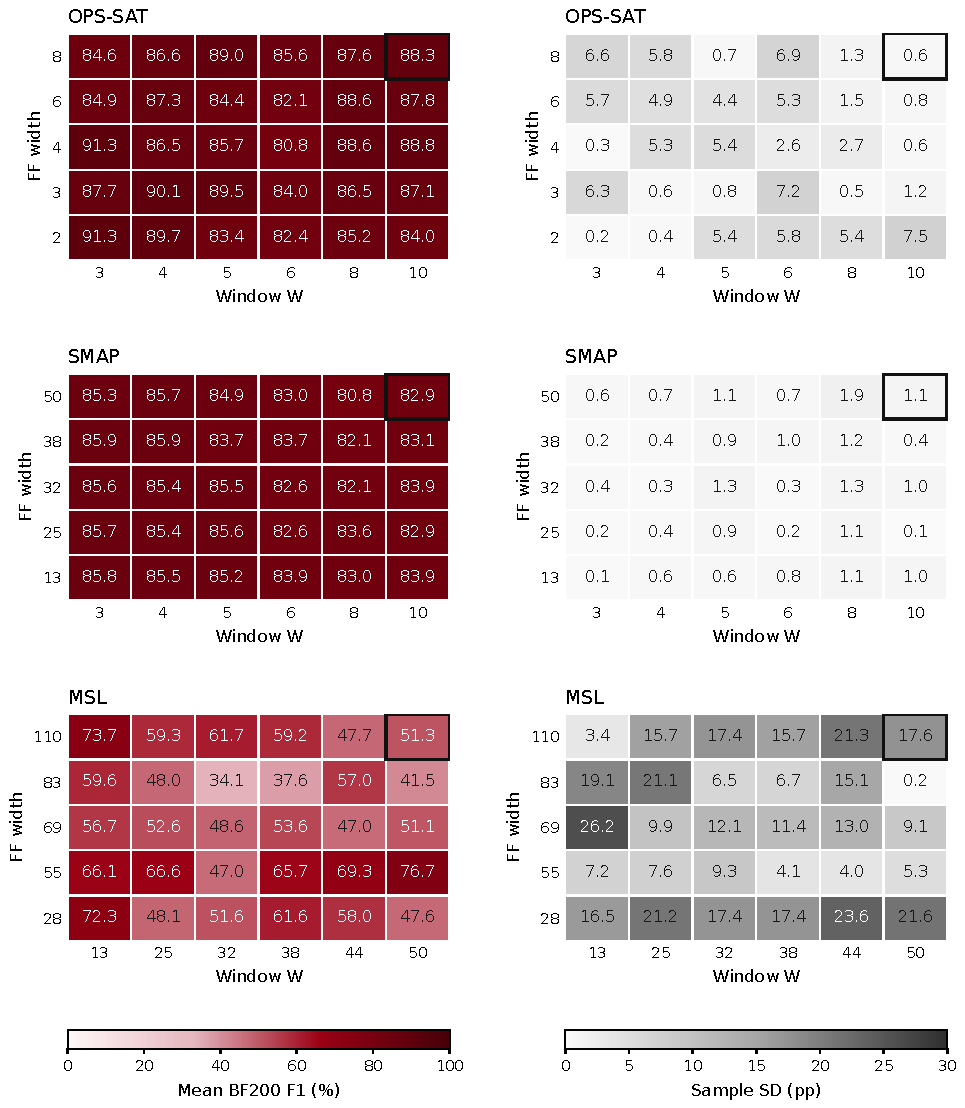
\includegraphics[width=\linewidth]{chapter5/grid_bf200.pdf}
  \caption{BF200 F1 over the complete window/width grid. Left panels show
  three-seed means in percent; right panels show sample standard deviations
  in percentage points at the same coordinates. Outlined cells are the
  largest-window, largest-width reference settings. Mean and variability
  scales are shared across datasets within their respective columns.
  The overview contains both recorded campaigns; the endpoint comparisons
  in Table~\ref{tab:ablation-endpoints} use the first campaign only.}
  \label{fig:ablation-grid}
\end{figure}
% Generated by scripts/plot_chapter5.py from verified data/chapter5/runs.csv.
% Left mean/right SD explicitly display uncertainty for each grid cell.

\section{Window-size reduction}
\label{sec:ablation-window}
The left column of Figure~\ref{fig:ablation-slices} varies the window while
holding feed-forward width at its largest value. This comparison shows
that shorter windows can be useful, but their effect depends on the
dataset and on threshold selection.

For \ac{OPS-SAT}, shortening the window from \num{10} to \num{3} at
width \num{8} lowers mean BF200 F1 from
\(\num{88.34}\pm\num{0.58}\) to
\(\num{84.59}\pm\num{6.61}\) percent. Mean \ac{POT} F1 increases
from \(\num{65.74}\pm\num{3.01}\) to
\(\num{72.31}\pm\num{22.51}\) percent, with a much wider seed spread.
The intermediate windows also depart from a monotonic trend. Window
reduction alone therefore does not establish a stable improvement on this
reference application.

For \ac{SMAP}, the same window change at width \num{50} raises mean
BF200 F1 from \SI{82.90}{\percent} to \SI{85.26}{\percent} and mean
\ac{POT} F1 from \SI{81.38}{\percent} to \SI{84.53}{\percent}.
The endpoint improvement is positive for each matched seed under both
methods. This is stronger evidence for a useful shorter-window setting,
although it is still conditional on the fixed dataset and evaluation
protocol.

For \ac{MSL}, shortening \num{50} samples to \num{13} at width
\num{110} raises mean BF200 F1 from \SI{51.26}{\percent} to
\SI{73.71}{\percent}. In contrast, \ac{POT} remains close to
\SI{85.6}{\percent} at both endpoints. The large BF200 change is not
mirrored by the alternative threshold method, so it should not be
interpreted as a threshold-independent improvement in detection.

A shorter window is not necessarily an information disadvantage for this
reconstruction task. The current sample remains in the encoder input and
the decoder query, as described in
Section~\ref{sec:background-tranadplus-training}. Reducing past context
therefore preserves direct access to the reconstruction target. It may
reduce interference from earlier conditions, while also reducing attention
work. This is a plausible computational explanation; the observed F1
values do not identify a physical correlation time in the telemetry.

\begin{figure}[htbp]
  \centering
  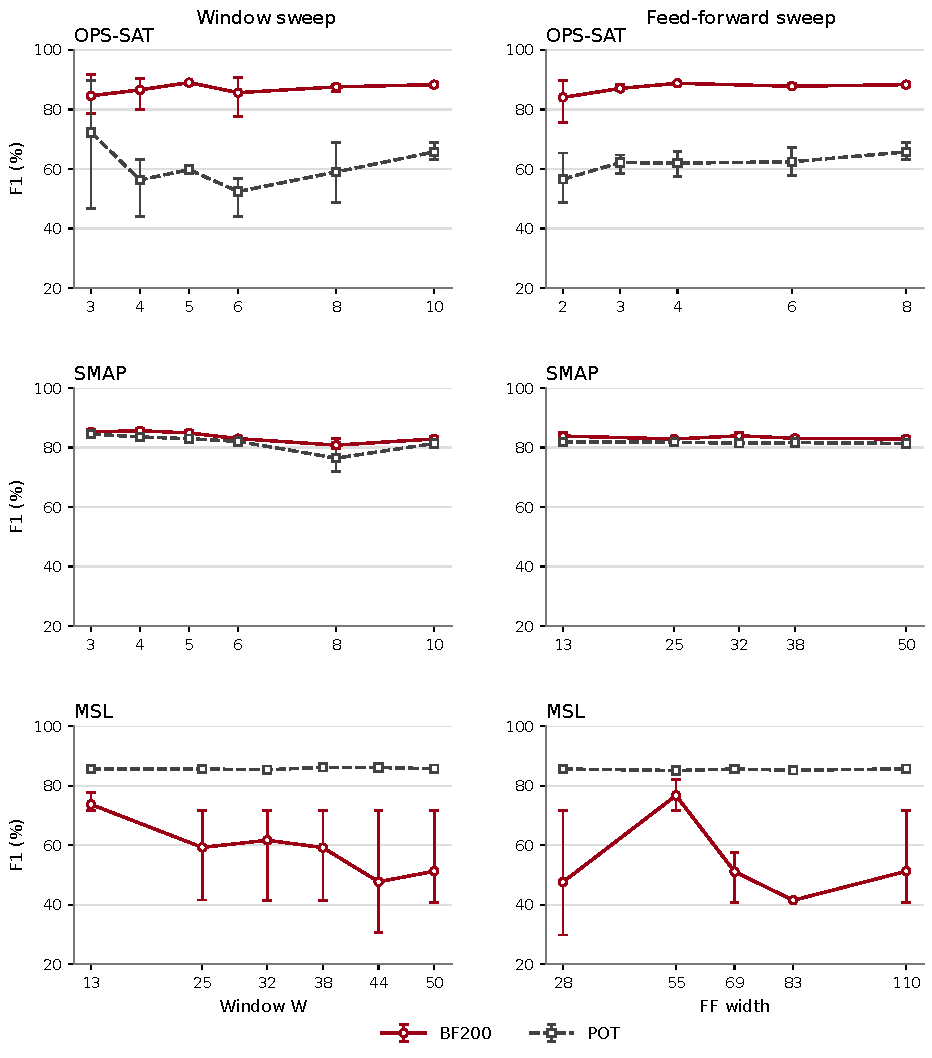
\includegraphics[width=\linewidth]{chapter5/slices_bf200_pot.pdf}
  \caption{Single-factor sweeps with point adjustment. Left: window length
  varies at the largest feed-forward width; right: feed-forward width
  varies at the largest window. The fixed widths are \num{8}, \num{50}
  and \num{110}, and the fixed windows are \num{10}, \num{10} and
  \num{50}, respectively, for \acs{OPS-SAT}, \acs{SMAP} and \acs{MSL}.
  Points are three-seed means; bars span the observed minimum and maximum.
  Lines connect sampled settings as visual guides. Both recorded campaigns
  contribute intermediate settings.}
  \label{fig:ablation-slices}
\end{figure}

\section{Feed-forward reduction}
\label{sec:ablation-feedforward}
The right column of Figure~\ref{fig:ablation-slices} holds the largest
window fixed and reduces the feed-forward width. Unlike window length,
this intervention directly reduces the number of learned weights.
The embedding width and attention-head count remain fixed, so it does
not shrink every part of the model.

For \ac{OPS-SAT}, reducing width from \num{8} to \num{2} at window
\num{10} lowers mean BF200 F1 from \SI{88.34}{\percent} to
\SI{84.05}{\percent}. Mean \ac{POT} F1 falls from
\SI{65.74}{\percent} to \SI{56.54}{\percent}.
The seed variability also increases. At this window length, the smallest
feed-forward map therefore has a measurable detection cost in the
recorded summaries.

For \ac{SMAP}, width \num{13} at window \num{10} gives BF200
\(\num{83.88}\pm\num{1.03}\) percent and \ac{POT}
\(\num{81.92}\pm\num{0.22}\) percent, compared with
\(\num{82.90}\pm\num{1.06}\) and
\(\num{81.38}\pm\num{0.98}\) percent at width \num{50}.
These changes are smaller than those produced by the window endpoints.
The sweep supports a substantial width reduction without a systematic
loss in these metrics.

For \ac{MSL}, \ac{POT} again stays near \SI{85.6}{\percent} as the
width changes. BF200 is much less stable: the largest and smallest widths
give \(\num{51.26}\pm\num{17.61}\) and
\(\num{47.62}\pm\num{21.56}\) percent. The intermediate width
\num{55} also behaves differently from neighboring widths in
Figure~\ref{fig:ablation-slices}. These observations do not support a
smooth monotonic relation between width and detection performance.

Reducing capacity can affect nominal and anomalous reconstruction errors
in different ways. A smaller reconstruction map can constrain which
patterns are reproduced, rather than merely increasing every error by
the same amount. As discussed in
Section~\ref{sec:background-reconstruction}, good reconstruction and good
anomaly separation are different objectives. The present comparisons
are consistent with that distinction, but do not by themselves demonstrate
that a wider model overfits.

\section{Joint reduction and interaction}
\label{sec:ablation-joint}
The joint endpoints reveal behavior that the isolated sweeps do not
predict. On \ac{OPS-SAT}, the smallest window and width together give
BF200 \(\num{91.28}\pm\num{0.18}\) percent and \ac{POT}
\(\num{88.49}\pm\num{0.85}\) percent. Both exceed the reference
means, although reducing either coordinate alone does not improve both
methods. The joint-minus-reference F1 differences are positive for all
three matched seeds under both threshold procedures.

We quantify this departure from additivity with an endpoint contrast:
\begin{equation}
  I_s = f_s(w_1,h_1)-f_s(w_1,h_0)-f_s(w_0,h_1)+f_s(w_0,h_0).
  \label{eq:ablation-interaction}
\end{equation}
Here, \(f_s(w,h)\) is F1 expressed in percent for the run with seed
\(s\), window \(w\) and feed-forward width \(h=d_{\mathrm{ff}}\). Subscripts \(0\)
and \(1\) denote the largest and smallest dimensions, respectively.
The contrast \(I_s\) is measured in percentage points. For \ac{OPS-SAT}
BF200, its mean and sample standard deviation are
\(\num{10.99}\pm\num{1.47}\) percentage points. This identifies a
nonadditive response of training and evaluation to the two interventions;
it is not a physical interaction parameter of the spacecraft.

For \ac{SMAP}, the joint endpoint gives BF200
\(\num{85.76}\pm\num{0.15}\) percent and \ac{POT}
\(\num{84.55}\pm\num{0.09}\) percent. Relative to the reference,
the mean changes are \num{+2.86} and \num{+3.17} percentage points,
respectively. Both changes are positive for every matched seed.
Most of the gain is already present after window reduction; adding width
reduction preserves it while further reducing parameter storage.

For \ac{MSL}, the joint \ac{POT} result is
\(\num{85.71}\pm\num{0.78}\) percent, almost unchanged from the
reference. BF200 has a higher mean but remains variable:
\(\num{72.26}\pm\num{16.53}\) percent. Its matched-seed changes
are \num{+48.45}, \num{-15.46} and \num{+30.02} percentage points.
The mean increase therefore does not represent an improvement in every
repetition. The defensible result is the preservation of \ac{POT}
performance at a lower computational cost, together with unresolved
BF200 sensitivity.
% Endpoint contrasts and seed differences: data/chapter5/evidence.json.

\section{Variability across datasets}
\label{sec:ablation-variability}
The standard deviations in Figure~\ref{fig:ablation-grid} are important
parts of the result. The \ac{SMAP} cells show comparatively small BF200
spread, while many \ac{MSL} cells have large spread. \ac{OPS-SAT}
contains both variable settings and a low-spread joint endpoint. A single
best seed would hide these differences.

Three seeds support descriptive variability, not a precise population
uncertainty estimate. A common seed initializes each experiment's random
generators, but different matrix shapes need not assign identical initial
weights to corresponding parameters. The train/test data and
\ac{OPS-SAT} split remain fixed, so the reported spread does not capture
uncertainty from acquiring another telemetry sample or another split.

Table~\ref{tab:ablation-operating-points} helps interpret the joint
endpoints. For \ac{OPS-SAT} BF200, mean precision rises from
\SI{87.02}{\percent} to \SI{94.25}{\percent}, while adjusted recall
falls slightly from \SI{89.80}{\percent} to \SI{88.50}{\percent}.
Under \ac{POT}, precision remains high and recall rises from
\SI{50.86}{\percent} to \SI{82.06}{\percent}.
The two methods therefore reach their F1 gains through different changes
in the selected operating point.

\begin{table}[htbp]
  \centering
  \small
  \setlength{\tabcolsep}{6pt}
  % Generated by scripts/prepare_chapter5.py from data/chapter5/runs.csv.
\begin{tabular}{@{}lllrrr@{}}
\toprule
Dataset & Setting & Method & Precision & Recall & AUC-PA \\
\midrule
\acs{OPS-SAT} & Reference & BF200 & \(\num{87.02}\pm\num{2.26}\) & \(\num{89.80}\pm\num{2.92}\) & \(\num{90.98}\pm\num{0.68}\) \\
\acs{OPS-SAT} & Reference & \acs{POT} & \(\num{93.10}\pm\num{0.51}\) & \(\num{50.86}\pm\num{3.47}\) & \(\num{74.34}\pm\num{1.75}\) \\
\acs{OPS-SAT} & Joint & BF200 & \(\num{94.25}\pm\num{0.28}\) & \(\num{88.50}\pm\num{0.45}\) & \(\num{92.68}\pm\num{0.17}\) \\
\acs{OPS-SAT} & Joint & \acs{POT} & \(\num{96.03}\pm\num{0.09}\) & \(\num{82.06}\pm\num{1.39}\) & \(\num{90.04}\pm\num{0.70}\) \\
\addlinespace
\acs{SMAP} & Reference & BF200 & \(\num{83.34}\pm\num{4.10}\) & \(\num{82.82}\pm\num{5.52}\) & \(\num{90.17}\pm\num{2.35}\) \\
\acs{SMAP} & Reference & \acs{POT} & \(\num{88.29}\pm\num{0.47}\) & \(\num{75.48}\pm\num{1.68}\) & \(\num{87.01}\pm\num{0.82}\) \\
\acs{SMAP} & Joint & BF200 & \(\num{91.87}\pm\num{0.22}\) & \(\num{80.40}\pm\num{0.21}\) & \(\num{89.68}\pm\num{0.10}\) \\
\acs{SMAP} & Joint & \acs{POT} & \(\num{88.88}\pm\num{0.05}\) & \(\num{80.62}\pm\num{0.17}\) & \(\num{89.57}\pm\num{0.08}\) \\
\addlinespace
\acs{MSL} & Reference & BF200 & \(\num{92.12}\pm\num{2.22}\) & \(\num{36.90}\pm\num{17.95}\) & \(\num{68.29}\pm\num{8.95}\) \\
\acs{MSL} & Reference & \acs{POT} & \(\num{79.13}\pm\num{0.15}\) & \(\num{93.44}\pm\num{0.43}\) & \(\num{95.30}\pm\num{0.21}\) \\
\acs{MSL} & Joint & BF200 & \(\num{92.44}\pm\num{1.72}\) & \(\num{61.45}\pm\num{22.96}\) & \(\num{80.44}\pm\num{11.39}\) \\
\acs{MSL} & Joint & \acs{POT} & \(\num{79.65}\pm\num{0.98}\) & \(\num{92.78}\pm\num{1.21}\) & \(\num{95.00}\pm\num{0.60}\) \\
\bottomrule
\end{tabular}

  \caption{Reference and joint-endpoint operating points. Entries are
  mean \(\pm\) sample standard deviation across \num{3} seeds, in percent.
  Each method retains the alpha and threshold selected for its own F1.
  AUC-PA uses the resulting adjusted binary predictions.}
  \label{tab:ablation-operating-points}
\end{table}

On \ac{SMAP}, BF200 precision also increases, while recall decreases
slightly at the joint endpoint. AUC-PA consequently need not rise with
F1: the two metrics combine the confusion counts differently. On
\ac{MSL}, the joint \ac{POT} precision and recall remain close to the
reference values, consistent with its nearly unchanged F1.

Threshold selection contributes to this interpretation. BF200 builds
its trial grid from the score minimum, mean and standard deviation.
Changes in score scale or extreme values can therefore change which
operating points are sampled. The large \ac{MSL} BF200 differences,
without comparable \ac{POT} differences, are consistent with sensitivity
to that finite search. They do not establish a corresponding gain in
continuous-score ranking. Point adjustment can additionally convert one
hit into detections over a labeled anomalous interval. Thus improved
adjusted F1 does not establish more accurate anomaly localization.

Feature count alone also cannot explain the dataset differences.
\ac{OPS-SAT} supplies one coordinate, while the \ac{SMAP} and
\ac{MSL} inputs contain a telemetry coordinate and command-related
coordinates, as discussed in Section~\ref{sec:datasets-smap-msl}.
Their counts of \num{25} and \num{55} are not counts of independent
physical sensors. The reconstruction score averages errors over all
input coordinates. In addition, embedding width is \(2F\), so reference
feed-forward width relative to embedding width is \num{4} for
\ac{OPS-SAT} and \num{1} for the native datasets. Input content,
relative capacity and annotation granularity change together.

The experiments therefore establish dataset-dependent detection--cost
trade-offs under a stated protocol. They do not isolate a physical
cause for each trend, and their absolute scores should not be used to
rank the intrinsic difficulty of the three missions.

\section{Detection performance and computational cost}
\label{sec:ablation-tradeoffs}
For the audited single-layer reference implementation, counting the
learned scalar parameters gives
\begin{equation}
  P(F,d_{\mathrm{ff}})=82F^2+47F+(12F+3)d_{\mathrm{ff}}.
  \label{eq:ablation-parameters}
\end{equation}
Here, \(P\) is the total trainable parameter count, \(F\) the input
feature count and \(d_{\mathrm{ff}}\) the feed-forward width; all are
dimensionless counts. The expression includes the shared encoder,
independent decoder stacks and shared output head. It matches the recorded
parameter totals for all \num{270} runs. It is a count for this
implementation, not a universal formula for Transformer models.
% Checked in scripts/prepare_chapter5.py against all model_statistics records.

The approximate matrix-operation counts of an encoder self-attention
block and its feed-forward layer scale as
\begin{equation}
  C_{\mathrm{attn}}=\mathcal{O}(w d^2+w^2d),
  \qquad
  C_{\mathrm{ff}}=\mathcal{O}(w d\,d_{\mathrm{ff}}).
  \label{eq:ablation-compute-scaling}
\end{equation}
Here, $w$ is the window length, $d=2F$ is the embedding width,
and $d_{\mathrm{ff}}$ is the feed-forward width. The expressions
include attention projections and pairwise products, and the
two feed-forward linear transformations. They are analytical
scalings, not latency measurements~\cite{Vaswani2017Attention,Sze2017EfficientDNN}.

The term proportional to \(F^2\) explains why reducing only the
feed-forward width removes a smaller fraction of parameters in the
multivariate models. Window length does not appear in
Equation~\eqref{eq:ablation-parameters}. Its reduction instead changes
attention and feed-forward work, as indicated by
Equation~\eqref{eq:ablation-compute-scaling}. The positional buffer
also changes size with the window, but is not learned weight storage.

\begin{table}[htbp]
  \centering
  \small
  \setlength{\tabcolsep}{5pt}
  % Generated by scripts/prepare_chapter5.py from data/chapter5/runs.csv.
\begin{tabular}{@{}llrrrr@{}}
\toprule
Dataset & Setting & Parameters & Weight KiB & MAC/window & Forward ms \\
\midrule
\acs{OPS-SAT} & Reference & \num{249} & \num{0.97} & \num{2124} & \(\num{1.835}\pm\num{0.004}\) \\
\acs{OPS-SAT} & Joint & \num{159} & \num{0.62} & \num{364} & \(\num{1.836}\pm\num{0.009}\) \\
\addlinespace
\acs{SMAP} & Reference & \num{67575} & \num{263.96} & \num{464700} & \(\num{1.783}\pm\num{0.034}\) \\
\acs{SMAP} & Joint & \num{56364} & \num{220.17} & \num{135500} & \(\num{1.809}\pm\num{0.011}\) \\
\addlinespace
\acs{MSL} & Reference & \num{323565} & \num{1263.93} & \num{11008140} & \(\num{1.858}\pm\num{0.031}\) \\
\acs{MSL} & Joint & \num{269199} & \num{1051.56} & \num{2297900} & \(\num{1.831}\pm\num{0.002}\) \\
\bottomrule
\end{tabular}

  \caption{Reference and joint-endpoint resources. Parameter counts,
  FP32 weight storage and matrix-multiplication MACs are computed quantities.
  Weight storage excludes buffers, optimizer state and file overhead;
  \num{1} KiB is \num{1024} bytes. Forward time is mean \(\pm\) sample
  standard deviation of the three seed-specific median latencies, measured
  at batch size \num{1} on an NVIDIA A100-PCIE-40GB. Each median uses
  \num{50} timed forwards after \num{10} warm-ups.}
  \label{tab:ablation-resources}
\end{table}

At the joint endpoints, learned parameter count falls by
\SI{36.14}{\percent} for \ac{OPS-SAT}, \SI{16.59}{\percent} for
\ac{SMAP} and \SI{16.80}{\percent} for \ac{MSL}.
Estimated matrix-multiplication work falls more strongly, by
\SI{82.86}{\percent}, \SI{70.84}{\percent} and
\SI{79.13}{\percent}, respectively. These operation counts cover the
two model passes, but exclude elementwise operations, softmax,
backpropagation and optimizer updates. They are not energy measurements.

The A100 timing results do not show proportional speedups. All reference
and joint means in Table~\ref{tab:ablation-resources} lie close to
\SI{1.8}{\milli\second}. Timing uses synchronized wall-clock intervals,
including model execution and launch/synchronization overhead, but excluding
score evaluation and data loading. Native timing inputs are synthetic
windows, whereas \ac{OPS-SAT} uses a real test window. These differences
and the batch-one execution regime limit cross-dataset timing comparisons.
% Source timing implementations: pipeline_metrics.py and opssat_pipeline.py;
% report measurement_settings; all records FP32, PyTorch2.8.0+cu128, A100.

Small models can be limited by fixed execution overhead rather than the
arithmetic removed by an intervention. The observations are consistent
with that possibility, but do not isolate a particular hardware
bottleneck. As discussed in Section~\ref{sec:datasets-resources}, reduced
parameter storage and arithmetic work remain separate findings from
measured latency or performance on an onboard device~\cite{Sze2017EfficientDNN}.

The useful trade-off is therefore not restricted to an accuracy penalty.
The joint \ac{OPS-SAT} and \ac{SMAP} settings reduce both learned storage
and estimated computation while increasing the recorded F1 means.
\ac{MSL} preserves \ac{POT} F1 with smaller resource requirements,
although BF200 remains unstable. These findings support simplification
within this experiment without implying that further reductions are
always beneficial.

\section{Implications for architectural simplification}
\label{sec:ablation-implications}
The first ablation stage identifies three practical directions. Window
length can remove arithmetic work without changing learned parameter
count. Feed-forward width changes parameter storage, but leaves a large
attention-related component in the multivariate models. Their effects
can interact, so studying one reduction in isolation is insufficient.

These observations motivate changes to the model structure itself.
Chapter~\ref{chap:architecture} examines a shared decoder stack, one
encoder--decoder pass, and an encoder with a reconstruction head, alongside
the unchanged reference, using the settings in
Table~\ref{tab:datasets-study-settings}. Such changes address repeated computation and
independent decoder parameters that remain after the present width and
window reductions. Their detection behavior must be measured rather than
inferred from parameter counts.


\chapter{Architectural Simplification}
\label{chap:architecture}

% Chapter outline; experimental prose remains to be written.

\section{Design hypotheses and model variants}
\label{sec:architecture-variants}
% Explain the component targeted by each implemented simplification and its expected cost.
% Do not preassign successful variants or introduce unimplemented model names.

\section{Training and evaluation of the variants}
\label{sec:architecture-protocol}
% Define appropriate training objectives and comparisons with the reference configurations.
% Record all changes accompanying a structural intervention, including loss changes.

\section{Anomaly-detection performance}
\label{sec:architecture-detection}
% Present OPS-SAT results and supporting SMAP/MSL comparisons with repeated seeds.

\section{Resource requirements and measured latency}
\label{sec:architecture-resources}
% Measure parameter/weight-memory changes and runtime under declared conditions.
% Weight sharing and removal of computation can have different resource effects.

\section{Detection--cost trade-offs and candidate configurations}
\label{sec:architecture-tradeoffs}
% Discuss candidates using an explicit selection protocol; retain negative findings.

\section{Limitations and implications for onboard inference}
\label{sec:architecture-onboard}
% State which efficiency claims are supported on the evaluated platform.
% Treat target-device deployment, power and radiation robustness as future work if untested.

\chapter{Quantization}
\label{chap:quantization}

% Separate chapter approved by the author on 2026-11-10.
% Outline only: no experimental conclusions are asserted here.
% Sources for subsequent writing: results/v16, results/v17, results/v18;
% tranad_plus/campaigns/precision and tranad_plus/campaigns/integer.

\section{Quantization methods and experimental protocol}
\label{sec:quantization-protocol}
% Identify parent checkpoints, datasets, architectures, configurations and seeds.
% Distinguish quantization schemes as well as storage and execution formats.

\section{Quantized weight storage and floating-point calculations}
\label{sec:quantization-weight-storage}
% Explain weight quantization followed by dequantization for FP32 computation.

\section{Integer matrix operations with quantized weights and activations}
\label{sec:quantization-integer-operations}
% Describe actual integer matrix products and the remaining floating-point steps.
% Distinguish four-bit operand precision from native INT4 hardware instructions.

\section{Anomaly-detection performance}
\label{sec:quantization-detection}
% Compare with paired FP32 parents under explicit threshold and PA protocols.

\section{Storage and computational requirements}
\label{sec:quantization-resources}
% Separate parameter counts, stored bytes, operation estimates and measured runtime.

\section{Limitations and implications for onboard inference}
\label{sec:quantization-onboard}
% State which results depend on the quantization scheme and evaluated platform.

\chapter{Discussion and Conclusions}
\label{chap:conclusions}

\todo[inline]{Outline approved; conclusions pending. Answer the research questions using the completed experiments. State limitations and the contribution to the initial TOAST activities without claiming untested onboard readiness.}

\section{Answers to the research questions}
\label{sec:conclusions-questions}
% Connect each answer to the baseline, ablation or architectural experiments.

\section{Main methodological and experimental findings}
\label{sec:conclusions-findings}
% Summarize reproducibility, evaluation sensitivity and supported simplification results.

\section{Limitations and validity of the conclusions}
\label{sec:conclusions-limitations}
% Discuss labels, threshold selection, fixed splits, seed variability and hardware scope.

\section{Future work within TOAST}
\label{sec:conclusions-outlook}
% Source: docs/papers/TOAST.pdf. Separate achieved work from later project objectives.
% Discuss deployment/compression and fault/radiation studies only as appropriate future work.

\backmatter
\phantomsection
\addcontentsline{toc}{chapter}{Bibliography}
\ifthesisbibliography
  \bibliographystyle{JHEP}
  \bibliography{references}
\else
  \chapter*{Bibliography}
  \noindent\emph{Add verified sources to references.bib and enable BibTeX in metadata.tex.}
\fi
\end{document}
